\documentclass[	%draft, % To display over/unterfull hboxes
				a4paper, % use DIN A4 Paper
				onecolumn, % Only one Column of text
				oneside, % Pint only right sides
				titlepage, % Print a titlepage
				openany, % Open new chapter on any page
				12pt] % Text size
				{report}

% set font to sans-serif
\renewcommand{\familydefault}{\sfdefault}

\usepackage[left=3.5cm,right=3.0cm,top=2cm,bottom=3cm]{geometry} % Page margins
\usepackage[ngerman]{babel} % Better line breaking
\usepackage[utf8]{inputenc} % Utf8 recognition
\usepackage[T1]{fontenc} % Translate from latex code to draw font
\usepackage{lmodern} % Bolder font
\usepackage{graphicx} % Display images
\usepackage{fancyhdr} % Header/footer
\usepackage[pdfborder={0 0 0}]{hyperref} % Links without visible lines
\usepackage[table]{xcolor} % Get the color in the table
\usepackage{pdflscape} % Get the table into landscape mode
\usepackage[lastpage]{zref} % Set a lable on the last page
\usepackage{listings} % Display formatted code
\usepackage{makeidx} % Generates the index
\usepackage{acronym} % Generates the list of abbreviations
\usepackage{multicol} % List of abbreviations with two columns
\usepackage{bibgerm} % BibTex German Style DIN 1505
\usepackage{longtable} % Multi page tables
\usepackage[onehalfspacing]{setspace}

% Tell LaTeX to generate an index
\makeindex

% No indent @ line start
\parindent 10pt
%\parskip2ex

% The bibstyle
% gerplain is for only numbers in alphabetic order
% geralpha is for name+year in alphabetic order
\bibliographystyle{gerplain}

% Header
\pagestyle{fancy}

\fancypagestyle{plain}{}
\fancyhead[RO,RE]{Seite \thepage\ von\reallastpage}
\fancyhead[LO,LE]{\leftmark}

% Set the lastpage counter -1 
% So the statutory declaration is not part of the page counter
\makeatletter
\newcommand{\reallastpage}{
  \the \numexpr \zref@extractdefault{LastPage}{page}{0}-1\relax
}
\makeatother

% Header for starting section
\fancypagestyle{rightmark}{
	\fancyhead[LO,LE]{\rightmark}
}

% Empty footer
\cfoot{}

% Brake long url in cite
\def\UrlBreaks{\do\/\do-}

% Suppress clubs (Schusterjungen) 
\clubpenalty = 10000

% Suppress widows (Hurenkinder)
\widowpenalty = 10000

% Suppress widows in front of a formular
\displaywidowpenalty = 10000

% Macro for centering extreme wide tables/figures
\makeatletter
\newcommand*{\centerfloat}{%
  \parindent \z@
  \leftskip \z@ \@plus 1fil \@minus \textwidth
  \rightskip\leftskip
  \parfillskip \z@skip}
\makeatother

%------------------------------------------------------------------------------
% Macro for reusing sume text:
%------------------------------------------------------------------------------

% Use to define some text and then re use the very same text
% \ref{sth:bla}
% \textlabel{Something AAA}{sth:bla}
\makeatletter
\newcommand*{\Textlabel}[2]{%
  \edef\@currentlabel{#1}% Set target label
  \phantomsection% Correct hyper reference link
  #1\label{#2}% Print and store label
}
\makeatother

%------------------------------------------------------------------------------
% Macro for the title:
%------------------------------------------------------------------------------

% The full title
\newcommand*{\Title}{\TitleFirstLine~\TitleSecondLine}

% Only the first line of the title
\newcommand*{\TitleFirstLine}{Betrachtung von Datensicherheit in E-Mail Systemen und Entwicklung eines SMTP-basierten Anonymisierungs-Algorithmus}

% Only the second line of the title
\newcommand*{\TitleSecondLine}{}

%------------------------------------------------------------------------------
% Macros for the list of abbreviations:
%------------------------------------------------------------------------------

% To wirte the text only once
\newcommand*{\ListOfAbbreviations}{Abkürzungsverzeichnis}

% use reversed form
\makeatletter
\renewcommand*{\@acf}[1]{%
\ifAC@footnote
\acsfont{\AC@acs{#1}}%
\footnote{\AC@placelabel{#1}\hskip\z@\AC@acl{#1}{} }%
\else
\acsfont{% Orig:\acffont
\AC@placelabel{#1}\hskip\z@\AC@acs{#1}%Orig: \AC@acl{#1}
\nolinebreak[3] %
\acfsfont{(\acffont{\AC@acl{#1}})}%Orig: (\acsfont{\AC@acs{#1}})
}%
\fi
\ifAC@starred\else\AC@logged{#1}\fi
}
\makeatother

%------------------------------------------------------------------------------
% Macros for the the Index:
%------------------------------------------------------------------------------

% The thickness of the line between the columns of the index and the list of 
% Abbreviations; 0.4 pt is the LaTeX standart
\newcommand*{\LineThickness}{0.4 pt}

% Display twoculums with  vertical seperator line
\makeatletter
\renewenvironment{theindex}
  {\if@twocolumn
      \@restonecolfalse
   \else
      \@restonecoltrue
   \fi
   \setlength{\columnseprule}{\LineThickness} % Thikness of the columnseprule
   \setlength{\columnsep}{35 pt}
   \begin{multicols}{2}[\chapter*{\indexname}] % Amount of Columns
   \markboth{\MakeUppercase\indexname}%
            {\MakeUppercase\indexname}%
   \thispagestyle{plain}
   \setlength{\parindent}{0pt}
   \setlength{\parskip}{0pt plus 0.3pt}
   \relax
   \let\item\@idxitem}%
  {\end{multicols}\if@restonecol\onecolumn\else\clearpage\fi}
\makeatother

%------------------------------------------------------------------------------
% Macros for table colors and longtables:
%------------------------------------------------------------------------------

% Table gray row
\newcommand*{\Grayrow}{\rowcolor{gray!35}}

% Table red cell
\newcommand*{\Redcell}{\cellcolor{red!30}}

% Table green cell
\newcommand*{\Greencell}{\cellcolor{green!30}}

% Generates a small empty row in a longtable
\newcommand*{\EmptyRow}{\multicolumn{0}{l}{} \\[-9pt]}

% Needs to be @ the end of the longtable, 
% generates a caption with correct spacing
% @par1: the text of the caption
\newcommand*{\CaptionLongtable}[1]
	{\multicolumn{0}{l}{} \\[-3pt]\caption{#1}}

%------------------------------------------------------------------------------
% Macros for quotes:
%------------------------------------------------------------------------------

% A direct quote
% @par1: The quoted text
% @par2: The source where the text is from
% @par3: The page where the text is from
\newcommand*{\QuoteDirect}[3]{\QuoteM{\emph{#1}} \cite[#3]{#2}}

% A direct quote without page
% @par1: The quoted text
% @par2: The source where the text is from
\newcommand*{\QuoteDirectNoPage}[2]{\QuoteM{\emph{#1}} \cite{#2}}

% A indirect quote
% @par1: The source where the text is from
% @par2: The page where the text is from
\newcommand*{\QuoteIndirect}[2]{(vgl. \cite[#2]{#1})}

% A indirect quote without page
% @par1: The source where the text is from
\newcommand*{\QuoteIndirectNoPage}[1]{(vgl. \cite{#1})}

% A reference
% @par1: The source where the text is from
\newcommand*{\RefIt}[1]{\cite{#1}}

% A text with quotation marks
% @par1: The text you want to quote
% »text«
\newcommand*{\QuoteM}[1]{\frqq #1\flqq}

% A text with single quotation marks
% @par1: The text you want to quote
% ›text‹
\newcommand*{\QuoteMs}[1]{\frq #1\flq}

% To adjust some words to the flow
% @par1: the adjusted words
% [text]
\newcommand*{\AdjustWords}[1]{{\normalfont[#1]}}

% Displays a reference to the given object
% @par1: the lable of the thing you want to see
% (Siehe auch Abbildung 1.1 »Ein Bild« auf Seite 4)
\newcommand*{\See}[1]
{(Siehe auch \autoref{#1} \QuoteM{\nameref{#1}} auf \autopageref{#1})}

% Displays a reference to an equation
% @par1: the lable of the equation you want to see
% (Siehe auch Gleichung 1.1 in »Dummy Section« auf Seite 5)
\newcommand*{\SeeEq}[1]
{(Siehe auch \autoref{#1} in \QuoteM{\nameref{#1}} auf \autopageref{#1})}

% The symbol for a elision
% Is used for more than missings one word or a sentence
% [...]
\newcommand*{\Elision}{{\normalfont[\dots]}}

% The symbol for a small elision
% Is used for only one missing word
% [..]
\newcommand*{\ElisionSmall}{{\normalfont[..]}}

% This is used if a book is cited at whole 
% passim means something like continuous
% text (vgl. [Aut99, passim]).
\newcommand*{\passim}{passim}

% To show the audience that there is something
% To display a wrong/importen part but not corrected in the quote
% text error [sic!] text
\newcommand*{\SIC}{{\normalfont[sic!]}}

% The text for a note from the author
% text, Anm. d. Autors
\newcommand*{\NoteFromAuthor}{{\normalfont\unskip , Anm. d. Autors}}

% Space btween \item in itemize
\newcommand*{\Itemizespace}{0 pt}

%------------------------------------------------------------------------------
% Listings:
%------------------------------------------------------------------------------

% Change the text from a listings caption
\renewcommand*{\lstlistingname}{Code}

% Change the text from the \autoref
\def\lstlistingautorefname{\lstlistingname}

% Change the text from the list of listings
\renewcommand*{\lstlistlistingname}{Codeverzeichnis}

\lstset{literate=%
    {Ö}{{\"O}}1
    {Ä}{{\"A}}1
    {Ü}{{\"U}}1
    {ß}{{\ss}}1
    {ü}{{\"u}}1
    {ä}{{\"a}}1
    {ö}{{\"o}}1
    {~}{{\textasciitilde}}1
}

\definecolor{lightgray}{rgb}{.9,.9,.9}
\definecolor{darkgray}{rgb}{.4,.4,.4}
\definecolor{purple}{rgb}{0.65, 0.12, 0.82}

\lstdefinelanguage{JavaScript}{
  keywords={typeof, new, true, false, catch, function, return, null, catch, switch, var, if, in, while, do, else, case, break},
  keywordstyle=\color{blue}\bfseries,
  ndkeywords={class, export, boolean, throw, implements, import, this},
  ndkeywordstyle=\color{darkgray}\bfseries,
  identifierstyle=\color{black},
  sensitive=false,
  comment=[l]{//},
  morecomment=[s]{/*}{*/},
  commentstyle=\color{purple}\ttfamily,
  stringstyle=\color{red}\ttfamily,
  morestring=[b]',
  morestring=[b]"
}

% C++ code environment
% @par1: The caption
% @par2: The label
% Used as:
%   \begin{c++}{caption}{label}
%      c++ code
%   \end{c++}
% Use empty brackets for code without caption and/or lable like:
%   \begin{c++}{}{} 
%      c++ code
%   \end{c++}
\lstnewenvironment{JavaScript}[2]{
	\lstset{ % General command to set parameter(s)
		language=JavaScript,
		% The language of the code
		basicstyle=\small \ttfamily,
		% The size of the fonts that are used for the code
		breaklines=true,
		% Sets automatic line breaking
		captionpos=b,
		% Sets the caption-position to bottom
		showstringspaces=false,
		% Underline spaces within strings only
		showspaces=false,
		% Show spaces everywhere adding particular underscores;
		% it overrides 'showstringspaces'
		keepspaces=true,
		% Keeps spaces in text, useful for keeping indentation
		% of code (possibly needs columns=flexible)
		numbers=left,
		% Where to put the line-numbers; 
		% possible values are (none, left, right)
		showtabs=false,
		% Show tabs within strings adding particular underscores
		keywordstyle=\bfseries \color{blue},
		% Keyword style
		rulesepcolor=\color{gray},
		% The color of the shadow of the box
		identifierstyle=\ttfamily,
		% The style for non-keywords
		commentstyle=\bfseries \color{gray},
		% Comment style
		stringstyle=\ttfamily \color{red!50!brown},
		% String literal style
		numberstyle=\tiny,
		% The style that is used for the line-numbers
		tabsize=2,
		% Sets default tabsize to 2 spaces
		frame=shadowbox,
		% Adds a frame around the code use single for no shadow
		rulecolor=\color{black},
		% If not set, the frame-color may be changed
		% on line-breaks within not-black text
		moredelim=[is][\underbar]{__}{__},
		% To create a underlind text to highlight something: __text__
		caption={#1},
		% The caption of the code example will be 
		% shown in the lstlistoflistings
		label={#2}
		% The lable used to make a ref to the code
	}
}{}

\lstnewenvironment{mail}[2]{
	\lstset{ % General command to set parameter(s)
		basicstyle=\small \ttfamily,
		% The size of the fonts that are used for the code
		breaklines=true,
		% Sets automatic line breaking
		captionpos=b,
		% Sets the caption-position to bottom
		showstringspaces=false,
		% Underline spaces within strings only
		showspaces=false,
		% Show spaces everywhere adding particular underscores;
		% it overrides 'showstringspaces'
		keepspaces=true,
		% Keeps spaces in text, useful for keeping indentation
		% of code (possibly needs columns=flexible)
		numbers=left,
		% Where to put the line-numbers; 
		% possible values are (none, left, right)
		showtabs=false,
		% Show tabs within strings adding particular underscores
		keywordstyle=\bfseries \color{blue},
		% Keyword style
		rulesepcolor=\color{gray},
		% The color of the shadow of the box
		identifierstyle=\ttfamily,
		% The style for non-keywords
		commentstyle=\bfseries \color{gray},
		% Comment style
		stringstyle=\ttfamily \color{red!50!brown},
		% String literal style
		numberstyle=\tiny,
		% The style that is used for the line-numbers
		tabsize=2,
		% Sets default tabsize to 2 spaces
		frame=shadowbox,
		% Adds a frame around the code use single for no shadow
		rulecolor=\color{black},
		% If not set, the frame-color may be changed
		% on line-breaks within not-black text
		moredelim=[is][\underbar]{__}{__},
		% To create a underlind text to highlight something: __text__
		caption={#1},
		% The caption of the code example will be 
		% shown in the lstlistoflistings
		label={#2}
		% The lable used to make a ref to the code
	}
}{}

\begin{document}



\thispagestyle{empty}
\begin{titlepage}
    \hrule
	\vspace*{3cm}
	\begin{center}
		{\Huge \sc \TitleFirstLine}

		\begin{Large}
			\vspace*{18pt}
			{\Large von Julian Ospald,\\
			geboren am 07.08.1986 in Bielefeld\\
			Betreut durch Frau Birgit Christina George}

			\vspace*{40pt}
			{\bf Bachelor-Abschlussarbeit},\\
			eingereicht am Fachbereich Campus Minden\\
			der FH Bielefeld, University of Applied Sciences\\
			
			\vspace*{20pt}
			\noindent{\today}
		\end{Large}
		
		\vspace*{40pt}
		
\includegraphics[scale=1.0]{Content/TitlePage/fhbi_logo_kompakt_orange}\\


	\vfill
    \hrule
   	\vfill

    
    		Copyright \copyright \ 2016 Julian Ospald <hasufell@hasufell.de>\\
Licensed under the \href{https://creativecommons.org/licenses/by-nc-sa/4.0/legalcode}{Attribution-NonCommercial-ShareAlike 4.0 International}.
	\end{center}
\end{titlepage}
\begin{abstract}
\thispagestyle{empty}

Im Angesicht globaler Überwachung durch Regierungen, %toref
schwer kontrollierbarer Sammlung und Speicherung von Benutzer-Daten durch Anbieter von Internetdiensten %toref
und fehlender Aufklärung über Konsequenzen internetbasierter Kommunikation soll diese Arbeit sowohl einen Überblick über aktuelle Probleme von E-Mail-Kommunikation, die die Privatsphäre des Benutzers betreffen, als auch eine Untersuchung möglicher Lösungen leisten.

Die Vielzahl möglicher Kommunikationsmittel im Internet erlaubt uns nicht, dieses Thema abstrakt zu behandeln. Oft unterscheiden sich diese fundamental: in der Art der Benutzung, dem verwendeten Protokoll, den zugrunde liegenden kryptografischen Algorithmen, den aktuellen Implementierungen und inhärenten Problemen.

Deshalb konzentriert sich diese Arbeit auf eines der ältesten digitalen Nachrichten- Übertragungsverfahren, welches schon im Arpanet %toref
erste Anwendung fand: die E-Mail. Dabei wird die E-Mail sowohl als Technologie aber auch als Kommunikationsform betrachtet und ihre Bedeutung aufgezeigt.

Der Überblick über aktuelle Probleme wird alle Aspekte behandeln, die relevant für die Privatsphäre des Benutzers sind. Dies beinhaltet konkrete Daten der Kommunikation wie Inhalt, aber auch Metadaten. %toexp: Meta-Daten

Bei der Betrachtung möglicher Lösungen werden zunächst bereits existierende aufgeführt, seien sie experimentell, schon implementiert oder nur konzeptionell. Nachfolgend wird ein alternativer Vorschlag inklusive Konzeption, rudimentärer Protokollbeschreibung, beinhaltender Algorithmen und Proof of Concept Implementierung der wissenschaftlichen Gemeinschaft zur Falsifikation unterbreitet.

Dieses Konzept soll als Idee, weniger als vollständige Lösung angesehen werden. Viele daraus folgende Probleme werden nicht ausreichend gelöst werden können. Diese werden jedoch nachfolgend untersucht und Vorschläge zur Weiterentwicklung unterbreitet.

Abschließend wird diskutiert, ob das vorgeschlagene Konzept ausreichend Potenzial hat, um bei entsprechender Weiterentwicklung eine angemessene Lösung sein zu können.

\end{abstract}


\setcounter{page}{3}
\tableofcontents

\chapter{Einleitung}
	Dieses Kapitel soll eine Übersicht über die Bedeutung, Beschaffenheit und Funktionsweise der E-Mail geben, was sowohl Protokolle und Format als auch in der Praxis relevante Technologien betrifft. Ebenso beschreibt es das Zusammenwirken dieser Protokolle und das daraus entstehende Gesamtsystem, welches auch grob die in der Praxis aufzufindende Server-Struktur umreißt. Dies ist notwendig, um die Problematik praktischer Anonymisierung und Verschlüsselung nachfolgend darzulegen, welche sowohl technologischer als auch ökosystematischer Natur sind.

Die E-Mail ist eines der ältesten digitalen Nachrichten-Übertragungsverfahren und wurde bereits im Arpanet über Erweiterungen des FTP Protokolls \QuoteIndirectNoPage{rfc196} \QuoteIndirectNoPage{rfc822}
angewendet. So gesehen entstand sie über einen längeren Zeitraum und entwickelte sich über mehrere RFCs über die Jahrzehnte.
Streng genommen bezeichnet die E-Mail jede Form briefähnlicher Nachrichten, die auf elektronischem Wege übertragen werden.

Das am häufigsten benutzte E-Mail System
setzt sich aus mehreren Komponenten zusammen, welche sehr stark miteinander korrelieren.
Die Basis hierbei bildet das IMF vom RFC 5322 \RefIt{rfc5322},
welches nur die Form einer Nachricht spezifiziert. Darauf aufbauend wurde das SMTP Protokoll im RFC 5321 \RefIt{rfc5321}
entwickelt, welches den Transport von Nachrichten spezifiziert. Weiterhin existieren Protokolle, die die Verwaltung und den Zugriff auf E-Mails durch den Benutzer, nicht deren Transport zwischen Servern, beschreiben. Dazu zählen POP3 nach RFC 1939 \RefIt{rfc1939}
und IMAP nach RFC 3501 \RefIt{rfc3501},
die sich allerdings in ihrer Funktionalität teilweise stark unterscheiden.

Konzeptionell besteht die gängige E-Mail in erster Linie aus einem äußeren Envelope, welcher Meta-Daten für den Transport beinhaltet. In diesem befinden sich Header und Body. Der Header beinhaltet ebenfalls Metadaten und die eigentliche Nachricht wird als Body bezeichnet.

Dieses System bildet allerdings nur die minimale Basis heutiger internetbasierter E-Mail Kommunikation und wird in der Praxis durch eine Vielzahl von Technologien erweitert. Manche davon wurden speziell als Erweiterungen für E-Mail Protokolle entwickelt, andere werden lediglich systemkompatibel eingesetzt.

Um die Relevanz heutiger E-Mail Kommunikation zu verstehen, ist es hilfreich Statistiken über Anzahl von E-Mail Konten und E-Mail Datenverkehr zu betrachten. Eine Studie der Radicati Group \RefIt{erep}
im Jahr 2013 ergab, dass sich die Anzahl weltweiter E-Mail Konten auf ca. 3.9 Mrd. beläuft. Die Prognose für das Jahresende 2017 sah einen Anstieg auf ca. 4.9 Mrd. Konten vor, welches einer jährlichen Wachstumsrate von 6\% entspricht. Ca. 24\% aller E-Mail Konten sind dieser Studie zufolge geschäftliche E-Mail Konten.
Der Datenverkehr insgesamt belief sich im Jahr 2013 auf ca. 182 Mrd. gesendeter E-Mails pro Tag. Es wird erwartet, dass dieses Volumen für geschäftliche E-Mails ansteigt. Zu bemerken ist allerdings, dass eine Abnahme des Volumens von Privatanwendern erwartet wird. Dies könnte laut der Radicati Group
an dem Aufkommen neuer Kommunikationstechnologien wie Instant Messaging und sozialen Netzwerken liegen.
Dennoch zeigen diese Zahlen, dass E-Mail Kommunikation äußerst relevant ist und sich als Kommunikationsform etabliert hat. \QuoteIndirect{erep}{S. 3, 4}

Aufgrund der hohen Verbreitung von E-Mail Kommunikation müssen auch Lösungen zur Anonymisierung diskutiert werden, die möglicherweise nicht optimal, aber mittelfristig praktikabel und kompatibel mit dem bestehenden System sind.

	\section{E-Mail Format (IMF)}
		Das im Kontext aktueller E-Mail Systeme benutzte E-Mail Format ist das \QuoteM{Internet Message Format}, kurz IMF.

Das IMF hat mehrere Versionen, angefangen beim RFC 822 \RefIt{rfc822},
welches noch den Titel \QuoteM{STANDARD FOR THE FORMAT OF ARPA INTERNET TEXT MESSAGES} trägt  und vom 13. August 1982 ist, bis hin zu RFC 2822 \RefIt{rfc2822},
welches bereits den Titel \QuoteM{Internet Message Format} trägt und vom April 2001 ist. Auf Basis dieser beiden RFCs wurde im Oktober 2008 der RFC 5322 \RefIt{rfc5322} veröffentlicht und ist damit die aktuellste Version zum Zeitpunkt dieser Arbeit. Das Ziel des RFC 5322 ist es eine Spezifikation für das Format von Text-Nachrichten, die zwischen Computer-Benutzern verschickt werden, bereitzustellen. Es ist im Kontext der E-Mail eingebettet und korreliert somit sehr eng mit dem SMTP Protokoll. Es beschreibt allerdings lediglich das Format der Nachrichten, nicht wie diese Nachrichten verschickt oder empfangen werden.

Das Format selbst setzt sich aus den Konzepten Header und Body zusammen. Der Header besteht aus mehreren Headerfeldern, welche jeweils einen Namen und einen Wert haben, die durch das Zeichen \verb-":"- getrennt werden. Die Headerfelder selbst werden durch einen Zeilenumbruch voneinander getrennt. Es gibt eine Reihe durch den RFC 5322 vordefinierter Headerfelder, die eine vorgegebene Bedeutung haben und von E-Mail Servern in bestimmter Weise verwertet werden. Dazu zählen vor allem folgende:
\begin{itemize}
\item \verb-From:- der Absender, beschrieben durch E-Mail Adresse, Name optional
\item \verb-To:- eine Liste von Empfängern, beschrieben durch E-Mail Adresse, Name optional
\item \verb-Date:- Zeitpunkt zu dem die Nachricht verfasst wurde, nicht Zeitpunkt des Transports
\item \verb-Subject:- Betreff der Nachricht
\item \verb#Message-ID:# eine von E-Mail Servern automatisch generierte ID wird intern benutzt, um mehrfache Zustellung zu verhindern
\item \verb#Received:# wird von E-Mail Servern, die nur weiterleiten, der Nachricht hinzugefügt, somit kann der Weg, den eine E-Mail nimmt, nachvollzogen werden
\end{itemize}
Die einzigen obligatorischen Headerfelder sind sind \verb-From:- und \verb-Date:-. Jeder Header, der diese Felder nicht besitzt, muss als nicht wohlgeformt zurückgewiesen werden. Weiterhin sind Headerfelder möglich, die nicht im RFC 5322 beschrieben sind. Diese können von E-Mail Servern ignoriert werden. Manche Headerfelder sind für E-Mail Clients gedacht oder werden zum Beispiel von Nachrichtenfiltern ausgewertet.
Dem Header folgt nach einer leeren Zeile der Body. Dieser besteht aus der eigentlichen Nachricht. Sowohl Header als auch Body sind auf 7-bit ASCII beschränkt.

Eine vollständige E-Mail gemäß IMF könnte z.B. so aussehen:
\\

\begin{minipage}{\linewidth}
\begin{mail}{E-Mail}{E-Mail}
From: Hans Bauer <hans@bauer.de>
To: Mina Meier <mina@meier.de>
Date: Tue, 8 Mar 2016 06:46:18 -0800
Subject: Beispiel-Mail
Message-ID: <18283.122131@bauer.de>
X-Mein-Header: True

Dies ist ein Beispieltext
über mehrere Zeilen.
\end{mail}
\end{minipage}
\\

Zeile 1 bis 6 stellen den vollständigen Header dar, getrennt durch die Leere Zeile 7. Der Body erstreckt sich über die Zeilen 8 bis 9.

Aufgrund der Beschränkungen dieses Systems auf 7-bit ASCII Zeichen und dem Fehlen von Inhalten, die nicht Text sind, wurde \QuoteM{Multipurpose Internet Mail Extensions}, kurz MIME, entwickelt. Es ist beschrieben in RFC 2045 \RefIt{rfc2045},
RFC 2046 \RefIt{rfc2046},
RFC 2047 \RefIt{rfc2047},
RFC 2049 \RefIt{rfc2049},
RFC 4288 \RefIt{rfc4288} und
RFC 4289 \RefIt{rfc4289}.
Die Integration dieses Systems in SMTP ist in RFC 1521 \RefIt{rfc1521}
und RFC 1522 \RefIt{rfc1522} beschrieben.

MIME erweitert den IMF Standard, indem es Zeichen erlaubt, die außerhalb des 7-bit ASCII Bereichs liegen, sowohl für den Body als auch für die Header. Weiterhin ermöglicht es Inhalte, die nicht Text sind, wie Programme, Audio-Dateien, Video-Dateien oder Bilder.
Anzumerken ist, dass MIME für unterschiedliche Protokolle verwendet wird, nicht nur für SMTP, sondern auch für beispielsweise HTTP \QuoteIndirect{Berjon:14:H}{Kapitel 4.7.10.3}.

Die Integration in den bestehenden IMF Standard erfolgt über neue dedizierte Headerfelder, die die nötigen Informationen beinhalten, um etwaige spezielle Headerfelder oder nicht-Text Teile des Bodies interpretieren zu können. Die relevanten Headerfelder lauten wie folgt:
\begin{itemize}
\item \verb#MIME-Version:# die Version des MIME Standards
\item \verb#Content-Type:# der Typ des Inhalts, z.b. \verb#text/plain#
\item \verb#Content-Disposition:# wurde in RFC 2183 \RefIt{rfc2183}
hinzugefügt und erlaubt das Angeben von sogenannten \QuoteM{Presentation Information}
\end{itemize}

Der MIME Standard erlaubt es aber vor allem sogenannte \QuoteM{MIME multipart messages} zu erstellen und zu interpretieren. Diese haben mehrere Bodies, die einzeln interpretiert werden. Getrennt werden diese durch das sogenannte \QuoteM{boundary}.

Eine E-Mail mit einem gewöhnlichen Datei-Anhang würde beispielsweise so aussehen:

\begin{minipage}{\linewidth}
\begin{mail}{MIME-Mail}{MIME-Mail}
From: Hans Bauer <hans@bauer.de>
To: Mina Meier <mina@meier.de>
Date: Tue, 8 Mar 2016 06:47:18 -0800
Subject: Beispiel-MIME-Mail
Message-ID: <18283.122131@bauer.de>
MIME-Version: 1.0
Content-Type: multipart/mixed;
 boundary="------------080209010109060601000409"

This is a multi-part message in MIME format.
--------------080209010109060601000409
Content-Type: text/plain; charset=utf-8
Content-Transfer-Encoding: 7bit

Mit Anhang.

--------------080209010109060601000409
Content-Type: text/plain; charset=UTF-8;
 name="Datei"
Content-Transfer-Encoding: base64
Content-Disposition: attachment;
 filename="Beispieldatei"

RGF0ZWlpbmhhbHQK
--------------080209010109060601000409--
\end{mail}
\end{minipage}
\\

Die ersten 8 Zeilen sind der E-mail Header, die 9. leere Zeile trennt Header und Body, welcher sich von Zeile 10 bis 25 erstreckt. Wichtig hierbei ist das Headerfeld \verb#Content-Type:# in Zeile 7, welches ankündigt, dass dies eine multipart MIME E-Mail ist. Ebenso gibt dieses Feld in Zeile 8 über \verb#boundary=# an, wo sich die einzelnen Teile im gesamten Body befinden. Dazu beinhalten die einzelnen Teile des Bodies erneut MIME Headerfelder, die eine korrekte Interpretation durch z.B. das E-Mail Programm vom Benutzer erlauben. So besitzt diese E-Mail einen gewöhnlichen Text-Anteil und einen Dateianhang, welcher Base64 verschlüsselt ist.

Dem Benutzer würde in diesem Fall im E-Mail Programm der Text \verb#Mit Anhang.# angezeigt werden und die Möglichkeit angeboten werden, die Datei mit dem Namen \verb#Beispieldatei# herunterzuladen.

	\section{E-Mail Protokolle}
		Dieses Unterkapitel behandelt die weitverbreiteten E-Mail Protokolle SMTP, POP3 und IMAP4, welche die Basis heutiger internetbasierter E-Mail Kommunikation bilden. Für diese Protokolle gibt es eine Vielzahl von Erweiterungen, die allerdings immer auf den bestehenden Protokollen aufbauen und diese selbst nicht verändern, damit die gemeinsame Schnittstelle nicht verloren geht.

Während das SMTP Protokoll die Kommunikation zwischen E-Mail Servern definiert, behandeln die Protokolle POP3 und IMAP4 die Verwaltung und den Zugriff auf E-Mails durch den Benutzer, nicht deren Transport zwischen Servern. Obwohl IMAP4 das modernere System ist,
verwenden viele Server noch POP3,
weshalb es hier der Vollständigkeit halber mit aufgeführt wird.
		\subsection{SMTP}
			Das SMTP Protokoll hat ähnlich wie das Internet Message Format mehrere Versionen, angefangen beim RFC 821 vom August 1982 \RefIt{rfc821}
über RFC 2821 vom April 2001 \RefIt{rfc2821}
bis hin zu RFC 5321 vom Oktober 2008 \RefIt{rfc5321},
welches die aktuellste Version zum Zeitpunkt dieser Arbeit ist. Das Ziel des RFC 5321 ist es, eine Spezifikation für ein Protokoll zum Transport von E-Mails auf Basis des IMF bereitzustellen. Somit beschreibt es die grundlegende Kommunikation von E-Mail Servern untereinander, inklusive Versand, Empfang, Fehlerbehandlung etc., als auch die Kommunikation zwischen einem SMTP Client, welcher eine E-Mail einreicht, und einem SMTP/E-Mail Server. Besonders hervorzuheben ist auch, dass dieser RFC nicht nur das SMTP Protokoll an sich beschreibt, sondern auch den \QuoteDirect{SMTP extension mechanism}{rfc5321}{S. 1, S. 9 ff}
und diverse praktische Gesichtspunkte, die über die Protokoll-Spezifikation hinausgehen.

In seiner Grundform beschreibt das SMTP Protokoll ein Verfahren, das aus mehreren Schichten besteht. Die erste Schicht ist hierbei die Verbindung selbst, gewöhnlicherweise zwischen einem SMTP Client und einem SMTP Server \QuoteIndirect{rfc5321}{S. 7}. Diese Verbindung wird generell über ein zuverlässiges Protokoll wie beispielsweise TCP hergestellt, da es keine Fehlertoleranz auf Daten-Ebene gibt. Sobald der Client sich mit dem Server verbunden hat, z.B. über das Programm \QuoteM{telnet}, stehen dem Client auf Verbindungsebene folgende Kommandos zur Verfügung:
\begin{itemize}
\item \verb#HELO:# identifiziert den Client zum SMTP Server
\item \verb#QUIT:# beendet die Verbindung zum SMTP Server
\end{itemize}

% TODO: EHLO, bzw. ESMTP

Wie hier zu erkennen ist, ist SMTP ein textbasiertes Protokoll. Beim Senden von \verb#HELO# muss der Client als Parameter seine FQDN mitschicken, erst danach ist die Verbindung erfolgreich zustande gekommen und der nächste Schritt ist möglich.

Hat die Verbindung diesen Zustand erreicht, so sind nachfolgend 0 oder mehr Transaktionen möglich, welches die nächste Schicht darstellt. Für eine einzelne Transaktion stehen dem Client folgende Kommandos zur Verfügung:
\begin{itemize}
\item \verb#MAIL FROM:# der erste Schritt, initiiert eine Transaktion und gibt den Sender der E-Mail an
\item \verb#RCPT TO:# der zweite Schritt, gibt den Empfänger an
\item \verb#DATA:# der gewissermaßen letzte Schritt gibt an, dass jetzt der Inhalt der E-Mail gemäß dem IMF folgt
\end{itemize}

Die weiteren Informationen auf Transaktions-Ebene wie \verb#MAIL FROM# und \verb#RCPT TO# in Verbindung mit der tatsächlichen E-Mail, die über das \verb#DATA# Kommando übermittelt wird, können auch grob als Envelope betrachtet werden.

Anzumerken ist hier, dass der E-Mail Server die Transaktion abbrechen muss, wenn diese Kommandos in fehlerhafter Reihenfolge ankommen. Die Reihenfolge ist genau einzuhalten, d.h. erst \verb#MAIL#, welches einmalig angegeben wird, dann \verb#RCPT#, welches mehrmals angegeben werden kann, dann \verb#DATA# und anschließend der Inhalt. Wenn der Inhalt der E-Mail gemäß IMF inklusive Header gesendet wird, so muss dieser mit einer Zeile enden, die nur einen Punkt enthält \QuoteIndirect{rfc5321}{S. 20}.

Nach jedem Kommando, das der Client sendet, muss der Server antworten. Dies geschieht über den Status-Code (engl. \QuoteDirect{reply code}{rfc5321}{S. 48 ff}), welcher aus 3 Ziffern besteht. Die erste Ziffer gibt an, ob die Antwort gut, schlecht oder unvollständig ist. Die zweite Ziffer gibt an, welche Art von Fehler vorliegt. Die dritte Ziffer gibt weitere Informationen über den Fehler an.
Eine vollständige Betrachtung der Status-Codes macht an dieser Stelle keinen Sinn, deshalb wird hier nur die erste Ziffer betrachtet, um einen groben Überblick zu verschaffen.
\verb#2xx# bedeutet, dass die Anfrage erfolgreich verarbeitet wurde und eine weitere Anfrage gesendet werden kann. \verb#3xx# bedeutet ähnlich wie \verb#2xx#, dass die Anfrage erfolgreich war, allerdings erwartet der Server jetzt noch weitere Informationen vom Client. Dies tritt beispielsweise beim \verb#DATA# Kommando auf, nach welchem der E-Mail Inhalt folgen muss. \verb#4xx# denotiert ein Kommando, das nicht akzeptiert wurde, was bedeutet, dass die Anfrage nicht ausgeführt wurde. Der Client kann bzw. sollte die Kommando-Sequenz wiederholen. \verb#5xx# denotiert ähnlich wie \verb#4xx# eine abgewiesene Anfrage. Allerdings ist dies ein permanenter Fehler und die zugrunde liegende Kommando-Sequenz sollte nicht wiederholt werden. Nach dem Status-Code folgt immer ein Text String, der menschenlesbar sein sollte. \QuoteIndirect{rfc5321}{S. 47 ff}.

Eine vollständige SMTP Sitzung könnte wie folgt aussehen (C steht für Client, S für Server):
\\
\\
\begin{minipage}{\linewidth}
\begin{mail}{SMTP-Sitzung}{SMTP-Sitzung}
C: telnet mail.wurst.de 25
S: 220 service ready
C: HELO wurst.de
S: 250 OK
C: MAIL FROM:<hans@bauer.de>
S: 250 OK
C: RCPT TO:<mina@meier.de>
S: 250 OK
C: RCPT TO:<wilhelm@keiser.de>
S: 250 OK
C: DATA
S: 354 start mail input
C: From: Hans Bauer <hans@bauer.de>
   To: Mina Meier <mina@meier.de>,
       Kaiser Wilhelm <wilhelm@keiser.de>
   Date: Tue, 8 Mar 2016 06:46:18 -0800
   Subject: Beispiel-Mail
   Message-ID: <18283.122131@bauer.de>
   X-Mein-Header: True
      
   Dies ist ein Beispieltext
   über mehrere Zeilen.
   .
S: 250 OK
C: QUIT
S: 221 closing channel
\end{mail}
\end{minipage}

Was hier besonders auffällt und äußerst wichtig für die weitere Betrachtung der Problematik und Implementierung sein wird, ist die Tatsache, dass die Headerfelder \verb#From# und \verb#To# auf Ebene des IMF praktisch losgelöst sind von den tatsächlich angegebenen Informationen \verb#MAIL FROM# und \verb#RCPT TO# auf Ebene des SMTP Protokolls. Sie können divergieren oder übereinstimmen. Obwohl es hier eine Reihe von Regeln gibt wie sich ein E-Mail Server verhalten soll, gibt es keine Garantie, dass hier Konsistenz herrscht. Dies wird unter anderem für das Headerfeld \verb#BCC# genutzt, welches angibt, dass die E-Mail an einen weiteren Empfänger gesendet werden soll, aber diese Information aus dem Header gelöscht wird, sobald der Server zustellt oder weiterleitet \QuoteIndirect{rfc5321}{S. 85}.

Ebenso ersichtlich in Zeile 1 ist hier, dass eine SMTP Sitzung generell über Port 25 abgewickelt wird \QuoteIndirect{rfc5321}{S. 68}. Reicht ein SMTP Client eine E-Mail bei einem Server ein, wird allerdings Port 587 gemäß dem RFC \QuoteDirect{Message Submission for Mail}{rfc6409}{S. 6} benutzt. Im Falle von SSL/TLS Verschlüsselung wird allerdings häufig Port 465 benutzt \QuoteIndirectNoPage{ssmtps}, obwohl nach RFC \QuoteDirect{SMTP Service Extension for Secure SMTP over TLS}{rfc2487}{S. 2} dafür kein designierter Port mehr vorhergesehen ist, da stattdessen STARTTLS benutzt werden soll.

\begin{figure}[htb]
	%\Centerfloat
	\centering
	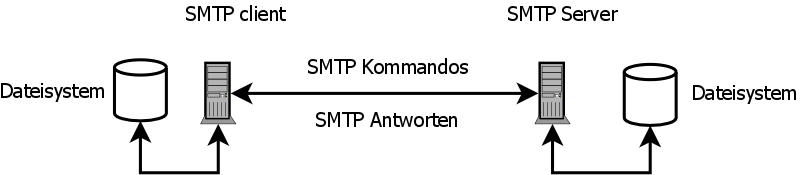
\includegraphics[scale=0.4]{Content/Intro/Protokolle/SMTP-Model.png}
	\caption{SMTP Modell}
	\label{fig:smtpmodel}
\end{figure}

		\subsection{POP3}
			POP3 ist die Version 3 des \QuoteM{Post Office Protocol}, spezifiziert in RFC 1939 \RefIt{rfc1939}. Während SMTP das Versenden, Erstellen und Weiterleiten von E-Mails beschreibt, beschreibt POP3 das Abholen, Auflisten und Löschen von E-Mails an einem E-Mail Server \QuoteIndirect{rfc1939}{S. 2}. Es ist keine Erweiterung des SMTP Protokolls, da es eine eigenständige Funktionalität hat, die SMTP nicht bereitstellt. Ebenso denkbar ist, dass POP3 mit einem E-Mail Server verwendet wird, der nicht SMTP zum Versenden benutzt, was allerdings in der Praxis kaum vorkommt. POP3 ist sehr simpel und eingeschränkt in der Funktionalität, was bereits in RFC 1939 angesprochen wird, mit einem Vermerk zu dem etwas mächtigeren IMAP4 Protokoll \QuoteIndirect{rfc1939}{S. 2}.

Ähnlich wie SMTP ist auch POP3 ein Client-Server basiertes System. In gängigen E-Mail Servern befindet sich also häufig nicht nur ein SMTP, sondern auch ein POP3 Server.

Ebenso wie SMTP ist auch POP3 TCP basiert. Die Kommunikation findet entweder über Port 110 \QuoteIndirect{rfc1939}{S. 3} statt oder im Falle von SSL/TSL Verschlüsselung über das POP3S Protokoll auf Port 995, welcher allerdings nach RFC 2595 \QuoteIndirect{rfc2595}{S. 9} als veraltet gilt und stattdessen STARTTLS auf dem Standardport 110 benutzt werden soll.

POP3 ist ein sehr zustandsbehaftetes Protokoll, d.h. die Verbindung kann sich in verschiedenen Zuständen befinden. Der erste Zustand ist der \QuoteDirect{AUTHORIZATION state}{rfc1939}{S. 3}, in dem sich die Verbindung befindet nachdem der POP3 server das sogenannte \QuoteDirect{greeting}{rfc1939}{S. 3} gesendet hat. Nachfolgend muss sich der Client authentifizieren. Ist die Authentifizierung erfolgreich, so gelangt die Verbindung in den \QuoteDirect{TRANSACTION state}{rfc1939}{S. 3}. In diesem Zustand kann der Client diverse Anfragen senden, um mit den auf dem POP3 Server liegenden E-Mails zu interagieren. Der letzte Zustand, der sogenannte \QuoteDirect{UPDATE state}{rfc1939}{S. 3 f}, wird erreicht nachdem der Client das \verb#QUIT# Kommando gesendet hat. In diesem Zustand werden alle Ressourcen freigegeben, die während des \QuoteM{TRANSACTION state} belegt wurden. Erst danach wird die TCP Verbindung geschlossen. \QuoteIndirect{rfc1939}{S. 3 f}

Dem POP3 Client stehen folgende Kommandos zur Kommunikation mit dem Server zur Verfügung:
\begin{itemize}

\item AUTHORIZATION state
\begin{itemize}
	\item \verb#USER <user>#: wird in Verbindung mit \verb#PASS# zur Authentifizierung verwendet, alternativ kann \verb#APOP# verwendet werden
	\item \verb#PASS <password>#: wird in Verbindung mit \verb#USER# zur Authentifizierung verwendet, alternativ kann \verb#APOP# verwendet werden
	\item \verb#APOP#: alternatives Authentifizierungsverfahren, welches das Passwort nicht als Klartext sendet
	\item \verb#QUIT#: beendet die Verbindung
\end{itemize}

\item TRANSACTION state
\begin{itemize}
	\item \verb#STAT#: Abfrage des Status der Mailbox
	\item \verb#LIST (i)#: zeigt Informationen zu der i-ten E-Mail oder zu allen E-Mails, gewöhnlicherweise Anzahl und Größe
	\item \verb#RETR i#: lädt die i-te E-Mail vom Server herunter
	\item \verb#DELE i#: löscht die i-te E-Mail
	\item \verb#NOOP#: tut nichts, der Server antwortet immer positiv
	\item \verb#RSET#: macht das löschen von E-Mails rückgängig
	\item \verb#TOP i l#: lädt den Header und die ersten l Zeilen der i-ten E-Mail herunter
	\item \verb#UIDL i#: zeigt die \QuoteM{unique-id} der E-Mail an
\end{itemize}

\item UPDATE state
\begin{itemize}
	\item \verb#QUIT#: beendet die Verbindung und führt mögliche \verb#DELE# Kommandos aus
\end{itemize}

\end{itemize}

Eine mögliche POP3-Sitzung könnte so aussehen:
\\
\\
\begin{minipage}{\linewidth}
\begin{mail}{POP3-Sitzung}{POP3-Sitzung}
S: <wartet auf Verbindung an TCP port 110>
C: <client verbindet sich>
S: +OK pop3.bauer.de POP3-Server
C: USER hans@pop3.bauer.de
S: +OK Valid user, now enter password
C: PASS <Klartext-Passwort>
S: +OK Password valid, maildrop locked and ready
C: STAT
S: +OK 500 4670
C: LIST 670
S: -ERR no such message
C: LIST 67
S: +OK 67 300
C: RETR 67
S: +OK 300 octets
S: <der POP3 server sendet die vollständige E-Mail>
S: .
C: DELE 67
S: +OK message 67 deleted
C: QUIT
S: +OK POP3 server signing off (maildrop empty)
C: <beendet Verbindung>
S: <wartet auf Verbindung an TCP port 110>
\end{mail}
\end{minipage}

Wie hier zu sehen ist, liegt ein impliziter Zustand vor, welcher aus dem Kontext erschlossen werden muss.

Wichtig anzumerken ist auch, dass das normale POP3 Authentifizierungsverfahren über die Kommandos \verb#USER# und \verb#PASS# unsicher ist, da die Daten als Klartext gesendet werden \QuoteIndirect{rfc1939}{S. 14}. Ebenso gilt das alternative APOP Authentifizierungsverfahren als unsicher \QuoteIndirect{apopinsec}{S. 1-18}.
Stattdessen kann STARTTLS mit POP3 verwendet werden, gemäß RFC 2595 \RefIt{rfc2595}.

		\subsection{IMAP4}
			IMAP4 ist die Version 4 des \QuoteM{INTERNET MESSAGE ACCESS PROTOCOL} spezifiziert in RFC 3501 \RefIt{rfc3501}. Es ist ähnlich wie POP3 ein textbasiertes Client-Server Protokoll, das das Auflisten, Löschen und Manipulieren von E-Mails an einem E-Mail Server erlaubt, weit über die Möglichkeiten von POP3 hinaus \QuoteIndirect{rfc1939}{S. 2}.

Ein E-Mail Server kann sowohl POP3 als auch IMAP4 gleichzeitig anbieten. Im Gegensatz zu POP3 erlaubt IMAP4 allerdings nicht nur E-Mails herunterzuladen, zu löschen oder aufzulisten, sondern direkt auf der Mailbox des E-Mail Servers zu operieren, was Funktionalitäten wie neue Ordner anzulegen erlaubt \QuoteIndirect{rfc3501}{S. 34 f} oder das serverseitige Durchsuchen von Nachrichten \QuoteIndirect{rfc3501}{S. 49 ff}.

Informationen werden nach Bedarf direkt vom IMAP4 Server abgerufen und nicht einzeln heruntergeladen. Deshalb ist auch im Gegensatz zu POP3 eine lokale Speicherung von Daten nicht notwendig, welche auch dazu führen kann, dass die lokale Mailbox von der entfernten Mailbox divergiert. E-Mail Programme bieten jedoch unabhängig von POP3/IMAP4 die Möglichkeit der lokalen Speicherung an, was allerdings Protokoll-agnostisch ist. Bei IMAP4 ist anzumerken, dass bei fehlender Internetverbindung und keiner expliziten lokalen Speicherung auf Programmebene der Zugriff auf E-Mails auch nicht mehr möglich ist.

IMAP4 benötigt ein zuverlässiges Netzwerkprotokoll wie beispielsweise TCP und wird über den Port 143 abgewickelt \QuoteIndirect{rfc3501}{S. 6}. Ist die Verbindung über IMAPS TLS/SSL-verschlüsselt wird häufig Port 993 benutzt, obwohl in RFC 2595 \RefIt{rfc2595} STARTTLS über den Standardport 143 beworben wird.

Ebenso wie POP3 ist auch IMAP4 ein zustandsbehaftetes Protokoll. Allerdings ist IMAP4 weitaus komplexer und kann sich in 4 verschiedenen Zuständen befinden. Wenn die Verbindung vom Client zum Server initial erstellt wurde, befindet sich die Kommunikation im \QuoteDirect{Not Authenticated State}{rfc3501}{S. 13}. Es wird vom Client nun erwartet, sich zu authentifizieren. Findet eine erfolgreiche Authentifizierung statt, so wird der \QuoteDirect{Authenticated State}{rfc3501}{S. 13} erreicht. Nachfolgend muss der Client eine Mailbox auswählen, bevor er weitere Kommandos zur Manipulation oder Einsicht von E-Mails abgeben kann. Ebenso wird dieser Zustand erreicht, wenn es einen Fehler beim Auswählen einer Mailbox gab oder nach einem erfolgreichen \verb#CLOSE# Kommando \QuoteIndirect{rfc3501}{S. 13}. Wurde eine Mailbox erfolgreich ausgewählt, so erreicht die Verbindung den \QuoteDirect{Selected State}{rfc3501}{S. 13}. In diesem Zustand kann auf der Mailbox operiert werden wie z.B. Ordner anlegen, E-Mails abrufen etc. Der letzte Zustand ist der \QuoteDirect{Logout State}{rfc3501}{S. 14} und kann aus allen vorherigen Zuständen erreicht werden. Hier wird die Verbindung terminiert.

Eine vereinfachte Darstellung der Kommunikation in einem SDL Diagramm ist in \autoref{fig:imap4} zu sehen. Diese Abbildung zeigt bereits die Komplexität des Protokolls, ist aber nicht vollständig. Deshalb kann an dieser Stelle aufgrund der Vielzahl möglicher Kommandos keine vollständige Betrachtung vorgenommen werden. Stattdessen wird nachfolgend eine einfache IMAP4 Sitzung betrachtet:

\begin{minipage}{\linewidth}
\begin{mail}{IMAP4-Sitzung}{IMAP4-Sitzung}
C: <öffnet Verbindung>
S: * OK IMAP4rev1 Service Ready
C: a001 login mrc secret
S: a001 OK LOGIN completed
C: a002 select inbox
S: * 322 EXISTS
S: * FLAGS (\Answered \Flagged \Deleted \Seen \Draft)
S: * 12 RECENT
S: * OK [UNSEEN 88] Message 88 is the first unseen message
S: a002 OK [READ-WRITE] SELECT completed
C: a003 fetch 8 body[header]
S: * 8 FETCH (BODY[HEADER] {342} 
S: From: Hans Bauer <hans@bauer.de>
S: To: Mina Meier <mina@meier.de>,
S:     Kaiser Wilhelm <wilhelm@keiser.de>
S: Date: Tue, 8 Mar 2016 06:46:18 -0800
S: Subject: Beispiel-Mail
S: Message-ID: <18283.122131@bauer.de>
S: X-Mein-Header: True
S:
S: )
S: a003 OK FETCH completed
C: a004 store 8 +flags \deleted
S: * 8 FETCH (FLAGS (\Seen \Deleted))
S: a004 OK +FLAGS completed
C: a005 logout
S: * BYE IMAP4rev1 server terminating connection
S: a005 OK LOGOUT completed     
\end{mail}
\end{minipage}

Wie hier zu sehen ist, sind die Transaktionen durchnummeriert und haben für Client und Server denselben Bezeichner. Der IMAP4 Zustand ist implizit und muss aus dem Kontext erschlossen werden.

% TODO: figure gets misplaced
% TODO: nicht alle server Nachrichten dargestellt
\begin{figure}[htb]
	%\Centerfloat
	\centering
	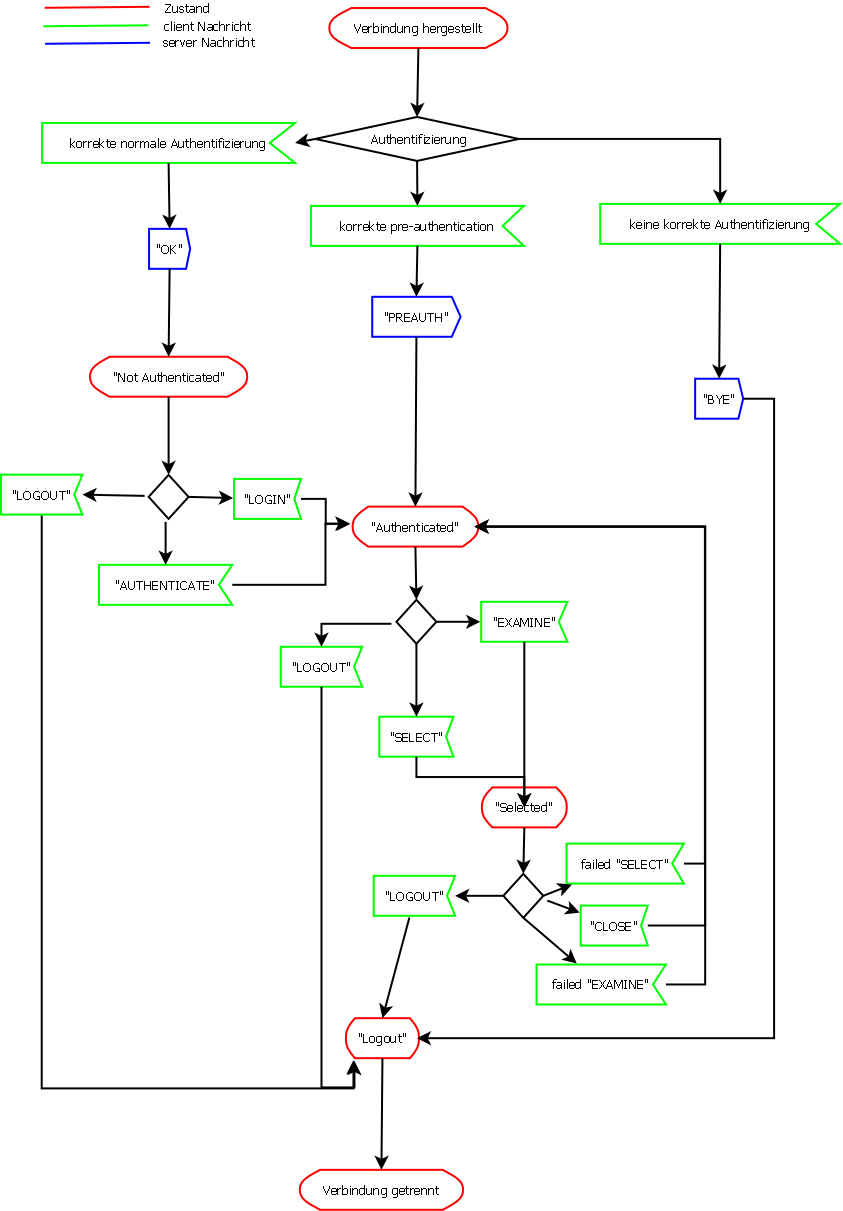
\includegraphics[scale=0.4]{Content/Intro/Protokolle/IMAP4.png}
	\caption{IMAP4 SDL Diagramm}
	\label{fig:imap4}
\end{figure}

\vfill
\clearpage

	\section{E-Mail als Gesamtsystem}
		Das hier vorgeschlagene System ist nicht nur eine SMTP-Erweiterung. Es handelt sich vor allem um eine Kombination aus bereits existierenden Technologien wie GPG, TorBirdy und TLS.

Selbst wenn für die SMTP-Erweiterung eine konkrete Spezifikation und eine funktionierende Implementierung existiert, muss der Benutzer dennoch weitere Schritte unternehmen, um dieses System korrekt zu benutzen. Dies erhöht die Wahrscheinlichkeit, dass das System inkorrekt benutzt wird.

Dies ist einerseits Dokumentationsarbeit, andererseits ist es aber auch denkbar, ähnlich wie Tor, eine Softwarelösung zur Verfügung zu stellen, die eine korrekte Konfiguration beinhaltet. Allerdings ist dies schwierig, da dies nur auf MUA Ebene möglich ist und der E-Mail Server immer noch fehlkonfiguriert sein kann.

Ebenso ist das Problem der SMTP Spezifikation ungelöst, welche keine Garantie gibt, dass 2 MTAs überhaupt verschlüsselt kommunizieren, selbst wenn beide dies beherrschen. Dies muss auf Implementierungsebene garantiert werden, für alle Komponenten, die in diesem Kryptografiesystem mitwirken.
	
\chapter{Motivation und Problematik}
	Wie durch Kapitel 1 erhellt wurde, sind die involvierten Protokolle für E-Mail Kommunikation äußerst verbose und übermitteln eine Menge an Metadaten und Inhaltsdaten. Standardmäßig werden alle diese Daten als Klartext übermittelt. Dazu gehören: Absender, Empfänger, Passwörter, Inhalt der E-Mail, etc. Dies bezieht sich auf nahezu alle Stationen, die eine E-Mail über das Internet durchläuft, mindestens aber folgende:
\begin{itemize}
\item MUA kommuniziert mit entfernten MSA
\item MTA kommuniziert mit entfernten MTA
\item MUA kommuniziert mit entfernten POP3/IMAP4 Server
\end{itemize}

Bei komplexeren Konfigurationen kann es sogar möglich sein, dass Informationen innerhalb einer Server-Konfiguration (z.B. entfernte Datenbank) sichtbar werden.

Um die Privatsphäre des Benutzers zu schützen, müssen so wenig Daten wie möglich und nur so viel wie nötig versendet werden. Die Daten, die gesendet werden müssen, sollten durch ein adäquates kryptografisches Verfahren verschlüsselt sein. Dies bezieht sich sowohl auf Metadaten als auch auf den Inhalt der E-Mail.

Nahezu alle existierenden Protokolle wie SMTP, IMAP4 und POP3 besitzen eine gewisse Unterstützung für kryptografische Methoden, die nachfolgend noch dargelegt werden. Allerdings können aufgrund der Beschaffenheit der genannten Protokolle immer noch Verbindungsdaten abgefangen werden, selbst wenn die Transaktionen (z.B. die SMTP Sitzung) kryptografisch verschlüsselt sind. Keines der existierenden E-Mail Protokolle bietet für letzteres eine adäquate Lösung. Dies ist nämlich das Problem der Anonymisierung von Metadaten, die nicht durch Verschlüsselung selbst versteckt werden können.

Anonymisierung von Metadaten in diesem Kontext unterscheidet sich also von der kryptografischen Verschlüsselung dadurch, dass, anstelle von Daten wie dem Inhalt einer Nachricht oder Transaktion, die Existenz der Transaktion oder Verbindung selbst für Außenstehende nicht nachvollziehbar ist, also die Verschleierung der Metadaten auf Netzwerkebene. Dies wird häufig über dedizierte Systeme erreicht, die über Routing-Algorithmen die Indirektion einer Verbindung vervielfachen. Diese Indirektion führt dazu, dass zum Nachvollziehen der Verbindung alle Stationen der Route bekannt sein müssen. Ein Beispiel eines solchen Algorithmus ist das \QuoteDirectNoPage{Onion Routing}{Syverson97anonymousconnections}.

Allerdings sind alle genannten Protokolle in der Lage, zumindest auf der Seite der kryptografischen Verschlüsselung etwas zu leisten.

Demnach liegt dieser Arbeit die Motivation zugrunde, das E-Mail System vor allem hinsichtlich der Anonymität für den Benutzer zu verbessern. Ob bestehende Systeme dies leisten können oder ob völlig neue Systeme entwickelt werden müssen, soll hier diskutiert werden.
In dem Zuge wird nachfolgend der aktuelle Stand der Verschlüsselung und Anonymität von E-Mail Kommunikation untersucht und die Anforderungen an eine adäquate Lösung formuliert.

		\section{Betrachtung von Datenschutz in aktuellen E-Mail Systemen}
			Dieser Abschnitt betrachtet den Datenschutz von aktuellen SMTP-basierten E-Mail Systemen hinsichtlich der Verschlüsselung und Anonymität.
			\subsection{Verschlüsselung von E-Mail-Verkehr}
				Mit Verschlüsselung sind kryptografisch-mathematische Methoden gemeint, um Nachrichten (z.B. Text) in eine neue Form zu bringen, die nicht ohne weiteres (z.B. ohne Schlüssel) in die ursprüngliche Form gebracht werden kann.

Bei der Betrachtung der Verschlüsselung von E-Mail Verkehr muss erst definiert werden welche Teile des Verkehrs verschlüsselt werden. Hier gibt es mehrere Schichten. Die erste Schicht sind die Inhaltsdaten der E-Mail, gewissermaßen der Body und eventuell auch die Header. Die zweite Schicht ist die Sitzung zwischen E-Mail Server und Client. Dies gilt für alle involvierten Protokolle SMTP, POP3 und IMAP4, die diese Verschlüsselung unterstützen müssen, um die einzelnen Kommandos vom Client zum Server und die Antworten vom Server zum Client über einen kryptografischen Kanal zu transferieren.

Zunächst werden Technologien bezüglich der Verschlüsselung des E-Mail Bodies betrachtet und nachfolgend Technologien auf Protokoll-Ebene untersucht. Dabei werden auch Probleme dieser Verfahren und Methoden aufgezeigt.

				\subsubsection{GPG}
					\QuoteDirectNoPage{GNU Privacy Guard}{gnupghp} ist eine vollständige und freie Implementierung des OpenPGP Standards, der in RFC 4880 \RefIt{rfc4880} definiert ist.

Es handelt hier sich um ein Verschlüsselungsverfahren, das asymmetrische Public-Key Verfahren mit symmetrischen Verfahren kombiniert \QuoteIndirect{rfc4880}{S. 1}.

Ein symmetrisches Verschlüsselungsverfahren benutzt nur einen einzigen Schlüssel für das Verschlüsseln und Entschlüsseln. Dieser muss also beiden Kommunikationspartnern zur Verfügung stehen, darf aber niemand anderem zugänglich sein. Die Übertragung eines solchen Schlüssels wird deshalb häufig über ein asymmetrisches Verschlüsselungsverfahren bewerkstelligt.
% toref

Ein asymmetrisches Public-Key Verfahren besteht auf Sender -und Empfänger-Seite jeweils aus einem Schlüsselpaar. Dieses setzt sich aus einem öffentlichen und einem privaten Schlüssel zusammen, die gemeinsam generiert werden. Nur die öffentlichen Schlüssel werden ausgetauscht und erlauben der jeweils anderen Partei für den Besitzer des Schlüsselpaars zu verschlüsseln. Der private Schlüssel wird vom Besitzer zum Entschlüsseln benutzt und kann mit einem Passwort geschützt sein.
% toref

\begin{figure}[htb]
	%\Centerfloat
	\centering
	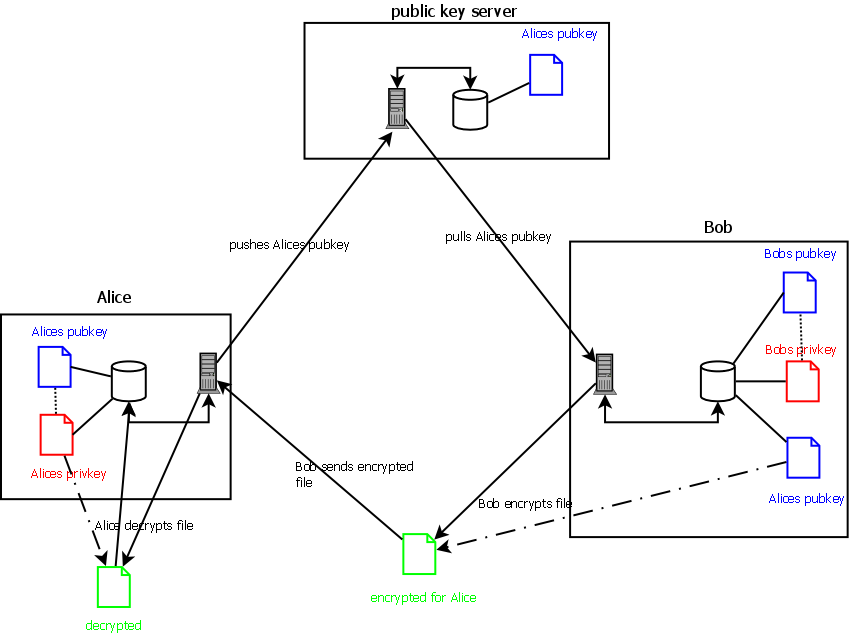
\includegraphics[scale=0.4]{Content/Problematik/BetrachtungDatenschutz/Verschluesselung/asymcrypto.png}
	\caption{Asymmetrisches Verschlüsselungsverfahren in der Praxis}
	\label{fig:asymcrypto}
\end{figure}

\autoref{fig:asymcrypto} stellt schematisch einen vereinfachten Ablauf einer verschlüsselten einseitigen Kommunikation von Bob zu Alice dar, basierend auf dem asymmetrischen Verschlüsselungsverfahren. Beide Parteien benötigen zunächst ein Schlüsselpaar, welches lokal generiert wird. Danach müssen die Parteien die benötigten öffentlichen Schlüssel austauschen. Dies kann manuell oder über einen öffentlichen Server geschehen. Als nächsten Schritt benutzt Bob den öffentlichen Schlüssel von Alice, um die Nachricht für Alice zu verschlüsseln. Dann verschlüsselt und sendet er diese. Anschließend benutzt Alice ihren privaten Schlüssel um die Nachricht zu entschlüsseln. \QuoteIndirect{Ferguson:2003:PC:862106}{Kapitel 3.3}

Hierbei kommt die Frage auf, woher Bob weiß, dass er den korrekten öffentlichen Schlüssel von Alice besitzt, wenn er diesen über einen öffentlichen Server geladen hat. Um dies festzustellen, wird ein \QuoteM{Secure Hash Algorithm} benutzt, der gewissermaßen den Fingerabdruck des öffentlichen Schlüssels darstellt. Bob kann nun Alice über einen sicheren Kanal kontaktieren (z.B. persönlich) und fragen, ob ihr Fingerabdruck des öffentlichen Schlüssels dem entspricht, den er lokal sieht. Aufgrund der Kollisionsunwahrscheinlichkeit von z.B. SHA-1 erlaubt dies eine sinnvolle Aussage über die Echtheit des öffentlichen Schlüssels, den Bob heruntergeladen hat. \QuoteIndirect{Ferguson:2003:PC:862106}{Kapitel 6.2.2}

GPG ist im Ablauf also ähnlich wie \autoref{fig:asymcrypto}, benutzt allerdings auch das symmetrische Verschlüsselungsverfahren in dem Verschlüsselungsprozess. Beim Sender wird dabei die Nachricht selbst lediglich über das symmetrische Verfahren mit einem einmaligen \QuoteM{session key} verschlüsselt. Dieser \QuoteM{session key} wird dann mit dem öffentlichen Schlüssel des Empfängers über das asymmetrische Verschlüsselungsverfahren verschlüsselt. Der symmetrische Schlüssel wird dann am Anfang der Nachricht mitgeschickt. Der Empfänger muss dann erst mit seinem privaten Schlüssel den \QuoteM{session key} entschlüsseln und dann mit diesem die eigentliche Nachricht. Dies geschieht natürlich auf Programmebene und wird nicht manuell vom Benutzer durchgeführt. \QuoteIndirect{rfc4880}{S. 6}

Anzumerken ist, dass GPG nicht nur für Verschlüsselung, sondern auch für Signierung benutzt werden kann. Damit kann der Absender einer Nachricht kryptografisch verifiziert werden. \QuoteIndirect{rfc4880}{S. 7}

GPG wird in der Praxis vielfältig benutzt. Dazu gehört das manuelle Verschlüsseln von Dateien für Andere, das Signieren von \QuoteM{git commits}
und das Verschlüsseln des Nachrichteninhaltes einer E-Mail.

Angenommen, die E-Mail selber ist über das SMTP Protokoll in sicherer Weise weitergeleitet worden, ohne dass ein Dritter diese verändern oder sehen konnte. Wenn die E-Mail auf dem Zielserver eintrifft, liegt sie dort dennoch als Klartext vor und wird durch die verschiedenen Komponenten innerhalb des Servers durchgereicht. Ist der E-Mail Server kompromittiert, so ist auch die Nachricht kompromittiert. Ist die Nachricht allerdings GPG-verschlüsselt, so ist dies nicht der Fall. Zumindest nicht für den Body.

			\subsubsection{TLS}
				TLS bezeichnet das Protokoll \QuoteM{Transport Layer Security}, welches im RFC 5246 \RefIt{rfc5246} definiert ist. Es ist ein Protokoll auf Applikationsebene, welches den Datenschutz und die Datenintegrität zweier kommunizierender Applikationen sicherstellen soll. Dabei besteht es aus zwei Schichten, einerseits aus dem \QuoteM{TLS Record Protocol} und dem \QuoteM{TLS Handshake Protocol}. \QuoteIndirect{rfc5246}{S. 4}

Das \QuoteM{TLS Record Protocol} stellt dabei die unterste Schicht dar, direkt über dem TCP Protokoll und stellt sicher, dass die Verbindung selbst verschlüsselt ist. Dies findet über ein symmetrisches Verschlüsselungsverfahren statt. Dabei ist der gemeinsame Schlüssel auf die Laufzeit einer Sitzung begrenzt. Ferner definiert dieses Protokoll wie die Integrität von Nachrichten über Hashfunktionen wie SHA-1 sichergestellt wird. \QuoteIndirect{rfc5246}{S. 4}

Das \QuoteM{TLS Handshake Protocol} hingegen ist im \QuoteM{TLS Record Protocol} eingebettet und übernimmt die Funktion der Authentifizierung. Auf dieser Ebene fällt ebenso die Entscheidung, welcher Verschlüsselungsalgorithmus benutzt wird und der Austausch der kryptografischen Schlüssel. Erst nach diesem Prozess wird die eigentliche Sitzung aktiv und Sitzungsdaten können gesendet werden. Dieser Prozess findet über asymmetrische Verschlüsselung basierend auf dem Public-Key Verfahren statt. Darauf basierend ist dann der Austausch des symmetrischen Sitzungsschlüssels sicher. \QuoteIndirect{rfc5246}{S. 4}

Der öffentliche Schlüssel des Servers wird in der Praxis häufig von einem weiteren öffentlichen Schlüssel einer sogenannten \QuoteM{Certificate Authority} signiert. Die verbindende Gegenstelle muss also nur dem Schlüssel der Certificate Authority vertrauen. Applikationen wie Webbrowser liefern häufig ein Paket von vertrauten Schlüsseln solcher Certificate Authorities mit. Öffentliche Schlüssel können allerdings auch \QuoteM{self-signed} sein ohne Verbindung zu einer Certificate Authority. Diese müssen dann allerdings beim Empfänger manuell verifiziert und zugelassen werden.
\QuoteIndirect{Ferguson:2003:PC:862106}{Kapitel 19 bis 21}

Die Schwächen und Probleme des TLS Protokolls und des darüber liegenden Zertifikats-Systems im einzelnen zu analysieren würde den Rahmen dieser Arbeit sprengen. Einige der bekannten Angriffe auf das Protokoll wurden in RFC 7457 \RefIt{rfc7457} veröffentlicht. Für einige davon existieren Lösungen, entweder durch Konfigurationsänderungen am Server-System oder durch Erweiterungen der TLS Spezifikation.
Festzuhalten ist aber lediglich, dass TLS das wohl am weitesten verbreitete Verfahren ist, um die Kommunikation im WWW, aber auch die Kommunikation von und zu E-Mail Servern zu verschlüsseln und das Problem eines \QuoteM{Man-in-the-Middle-Angriff}, kurz MITMA \RefIt{mitm}, zu lösen.

Die Protokolle SMTPS, POP3S und IMAPS sind also nur Bezeichner für die Protokolle SMTP, POP3 und IMAP, die auf den dedizierten Ports 465, 995 und 993 ansprechbar sind und nur über das TLS Protokoll ansprechbar sind. Für diese existiert keine konkrete Spezifikation.


			\subsubsection{STARTTLS}
				STARTTLS ist eine Erweiterung für eine Reihe von Text-basierten Protokollen wie IMAP, POP3 und SMTP, aber auch FTP oder LDAP. Für IMAP und POP3 wurde diese in RFC 2595 \RefIt{rfc2595} definiert und für SMTP in RFC 3207 \RefIt{rfc3207}. Die Erweiterung benutzt das TLS Protokoll, hat aber im Vergleich zu einer gewöhnlichen TLS Kommunikation ein paar entscheidende Unterschiede:
\begin{itemize}
\item die Verbindung wird zunächst unverschlüsselt initiiert
\item nach der Begrüßung antwortet der Server, dass er über STARTTLS verfügt und der Client kann eine TLS verschlüsselte Verbindung initiieren und anschließend z.B. Logindaten senden
\item es wird kein dedizierter SSL Port benötigt
\item STARTTLS ist allerdings protokollspezifisch
\end{itemize}

Nachfolgend eine SMTP-basierte STARTTLS Verbindung:
\begin{mail}{SMTP-STARTTLS}{SMTP-STARTTLS}
S: <wartet auf TCP Port 25>
C: <öffnet Verbindung>
S: 220 service ready
C: EHLO bauer.de
S: 250-bauer.de welcome
S: 250-STARTTLS
C: STARTTLS
S: 220 Go ahead
C: <startet TLS Verhandlung>
C & S: <Verhandlung einer TLS Sitzung>
C & S: <Überprüfen des Ergebnisses>
...
\end{mail}

Ab Zeile 12 ist die Verbindung verschlüsselt und der Server kann beispielsweise über \verb#AUTH PLAIN# eine Klartext-basierte Authentifizierung anfordern, da diese nun innerhalb der verschlüsselten Verbindung sicher ist.

Die Vorteile von STARTTLS sind einmal, dass keine zusätzlichen Ports benötigt werden, aber auch, dass optional eine unverschlüsselte Verbindung weitergeführt werden kann. Da dies aber häufig unerwünscht ist, ist es bedingt möglich den Server so zu konfigurieren, dass eine nachfolgende TLS Verbindung erforderlich ist \QuoteIndirect{rfc2595}{S. 3} \QuoteIndirect{rfc3207}{S. 3}. Für POP3/IMAP in Verbindung mit STARTTLS müssen Server so konfigurierbar sein, dass eine erfolgreiche TLS Verbindung etabliert sein muss, bevor jede Art von Benutzerauthentifizierung stattfindet \QuoteIndirect{rfc2595}{S. 3}. Auf SMTP Ebene ist es nur für Server erlaubt, die nicht \QuoteDirect{publicly-referenced}{rfc3207}{S. 3} sind, TLS Verschlüsselung zu erzwingen.

Zu den Nachteilen gehört allerdings, dass bei STARTTLS mehr Metadaten verbreitet werden als bei direkter TLS Verbindung auf einem alternativen Port. Da die Verbindung initial unverschlüsselt ist, erlaubt dies auch weitere Angriffsvektoren wie z.b. \QuoteDirect{STARTTLS Command Injection Attack (CVE-2011-0411)}{rfc7457}{S. 4}, bei denen u.a. versucht werden kann, die Verbindung während der kurzen Periode von Klartextkommunikation herunterzustufen, indem das \verb#STARTTLS# Kommando vom Client gar nicht erst den Server erreicht. Dies hängt aber auch wie schon eingangs erwähnt von der Serverkonfiguration ab. Ebenso sagt die Spezifikation nicht aus wie ein Client sich exakt zu verhalten hat, wenn eine STARTTLS Verbindung fehlschlägt: \QuoteDirect{If the TLS negotiation fails or if the client receives a 454 response, the client has to decide what to do next.  There are three main choices: go ahead with the rest of the SMTP session, retry TLS at a later time, or give up and return the mail to the sender.}{rfc3207}{S. 6}.
Dies bedeutet, dass der Client theoretisch versuchen kann, mit einer Klartext-Verbindung fortzufahren.
Dies muss auf Clientebene gelöst werden und entsprechende Konfigurationsoptionen angeboten werden, ist aber nicht garantiert.

Trotz der genannten Probleme ist STARTTLS das einzige Protokoll, das einen TLS-basierten Verbindungsaufbau von SMTP, POP3 und IMAP Servern überhaupt spezifiziert, im Gegensatz zu den Pseudoprotokollen SMTPS, POP3S und IMAPS, die keine konkrete Spezifikation haben und das Verhalten zwischen Client und Server demnach von Implementierungsdetails abhängt.

		\subsection{Anonymität von E-Mail-Verkehr}
			Wie bereits erwähnt bezeichnet Anonymität im Kontext dieser Arbeit das Verschleiern von Metadaten. Nicht immer ist die Trennung von Inhaltsdaten und Metadaten streng nachvollziehbar. So ist es beispielsweise diskutierbar, ob die allgemeinen Informationen einer SMTP Sitzung ohne Betrachtung der E-Mail Nachricht selbst als Metadaten gelten. Als Metadaten im Kontext dieses Kapitels sind aber vor allem Verbindungsdaten wie IP-Adressen gemeint.

Das SMTP Protokoll sowie die Protokolle POP3 und IMAP liefern über ihre Spezifikation keinerlei Methoden eine solche Anonymisierung durchzuführen. Ebenso sind keine Protokoll-Erweiterungen bekannt, die dieses leisten.

Allerdings sind protokollunabhängige Lösungen möglich. Eine davon ist die MUA-Erweiterung \QuoteM{TorBirdy}.

			\subsubsection{TorBirdy}
					\QuoteM{TorBirdy} \RefIt{torbirdyhp} \RefIt{torbirdy} ist eine Erweiterung für den MUA \QuoteDirectNoPage{Mozilla Thunderbird}{thunderbirdhp} mit dem Ziel die Kommunikation folgender Komponenten zu anonymisieren:
\begin{itemize}
\item MUA kommuniziert mit entfernten MSA
\item MUA kommuniziert mit entfernten POP3/IMAP4 Server
\end{itemize}

Dies sind zwei von den eingangs drei erwähnten Angriffspunkten.

Das Prinzip von TorBirdy ist, den gesamten Datenverkehr der Kommunikation von Thunderbird mit dem E-Mail Server über das Tor-Netzwerk \RefIt{torpaper} zu leiten.

Das Tor-Netzwerk selbst ist allerdings abstrakter als dieser Anwendungsfall. Es erlaubt allgemein das Anonymisieren von TCP-Verbindungen jeglicher Art. Dieses wird wiederum auf Basis des \QuoteM{Onion Routings} \RefIt{onionrouting1} \RefIt{onionrouting2} realisiert. Das Onion Routing läuft grob in folgenden Schritten ab \QuoteIndirectNoPage{onionrouting2}:
\begin{enumerate}
\item der initiale Sender wählt von einem sogenannten Verzeichnisserver (engl. \QuoteM{directory node}) eine geordnete, aber zufällige Liste von Knoten aus, welche den Pfad bilden, den die Daten bis zum schlussendlichen Empfänger nehmen
\item vom Verzeichnisserver wird ein öffentlicher Schlüssel (asymmetrisches Verschlüsselungsverfahren) für den ersten Knoten bezogen, der sogenannte Eintrittsknoten (engl. \QuoteM{entry node})
\item eine Verbindung wird hergestellt und ein Sitzungsschlüssel (symmetrisches Verschlüsselungsverfahren) erstellt
\item über die erstellte Verbindung kann der Sender eine Nachricht an einen zweiten Knoten senden, die allerdings mit dessen öffentlichem Schlüssel verschlüsselt wurde und somit nicht vom Eintrittsknoten entschlüsselt werden kann
\item der zweite Knoten verbindet sich dazu mit dem ersten Knoten und ist somit indirekt mit dem Sender verbunden, ohne davon Wissen zu haben
\item diese Verbindung kann jetzt zu einem dritten, vierten, usw. ... Knoten erweitert werden
\item der schlussendliche Empfänger benutzt dieselbe Reihe von Knoten zurück zum Sender, nur umgekehrt
\end{enumerate}

Dieses Konzept wird \QuoteM{Onion Routing} genannt, da hier eine verschachtelte Verschlüsselung vorliegt, die nach und nach beim Weiterreichen an den jeweils nächsten Knoten wie eine Zwiebel geschält wird. Die Nachrichten für jede Schicht sind mit dem öffentlichen Schlüssel für exakt diese Schicht verschlüsselt, sodass kein Knoten in der Mitte den vollständigen Pfad herausfinden kann.
Zu jedem Zeitpunkt hat jeder Knoten nur Wissen über den vorherigen Knoten und den nachfolgenden Knoten. Der erste Knoten ist immer der Eintrittsknoten und der letzte der Austrittsknoten (engl. \QuoteM{exit node}). Die Verbindungspfade werden im Tor-Netzwerk in regelmäßigen Abständen geändert. Das Tor-Netzwerk selber benutzt intern konsistent TLS Verschlüsselung.

Dieses Konzept wird vor allem im WWW benutzt, über den sogenannten \QuoteM{Tor Browser} \RefIt{torbrowserhp}.
TorBirdy macht allerdings in derselben Weise Gebrauch davon, bleibt aber kompatibel mit den Protokollen SMTP, POP3 und IMAP.

Anzumerken ist, dass der Versand von E-Mails auch über Weboberflächen möglich ist und somit eine gewöhnliche Verbindung über den Tor Browser verwendet werden kann. Allerdings gibt es auch diverse Gründe dies für vollwertige MUAs zu ermöglichen \QuoteIndirect{torbirdy}{S. 4}.

		\subsection{Bewertung}
			Nahezu alle Datenschutzmechanismen für E-Mails sind erst wesentlich später als die ursprünglichen Protokolle wie SMTP entstanden und haben sich mit der Zeit entwickelt. Viele der vorgestellten Technologien sind unabhängige Lösungen, die lediglich in Verbindung mit E-Mail Systemen verwendet werden können, andere sind wiederum Protokollerweiterungen, die sich mehr oder weniger sinnvoll in das Gesamtkonzept einfügen. Sichtbar anhand der untersuchten Technologien ist allerdings, dass hier keine konsistente Lösung vorliegt. Jede Lösung zielt auf einen anderen Bereich ab und versucht ein atomares Problem zu lösen, ohne dabei auf die Kohärenz eines in der Praxis eingesetzten E-Mail Systems achten zu können. Dies öffnet unabhängig vom Kohärenzproblem auch das Problem der Konfiguration eines konkreten Systems. Die immense Komplexität der zusammenspielenden Komponenten wurde in Kapitel 1 erhellt und ist ein praktisches Problem solcher Systeme.

Dennoch ist es möglich die genannten Systeme zu nutzen, um eine Reihe von Problemen bezüglich Datensicherheit zu lösen. Um die Inhaltsdaten des Bodies einer E-Mail für jeden außer der Empfängerperson unzugänglich zu machen, kann das asymmetrische Verschlüsselungsverfahren GPG benutzt werden. Selbst der Server-Betreiber oder ein Man-in-the-Middle ist dann nicht in der Lage, die E-Mail ohne weiteres zu entschlüsseln, unabhängig davon, in welcher Weise diese transportiert wurde. Allerdings bezieht sich GPG nur auf den Body einer E-Mail und nicht auf die Header. Ebenso ist es möglich, die Protokoll-Transaktionen von SMTP, POP3 und IMAP über direktes TLS oder STARTTLS zu verschlüsseln. Problematisch hierbei ist aber, dass eine verschlüsselte Verbindung nicht durchgängig garantiert werden kann, z.b. wenn die Verbindung über mehrere MTAs geht oder wenn der E-Mail Server erlaubt zu unverschlüsselten Verbindungen herunterzustufen, insbesondere über SMTP STARTTLS. Und letzten Endes ist eine gewisse Anonymisierung der IP-Verbindungsdaten über TorBirdy möglich. Diese gilt allerdings nur für die Kommunikation des MUA mit dem MSA bzw. POP3/IMAP server.

\autoref{fig:bewertung} zeigt sehr deutlich, dass selbst beim Einsatz all dieser Technologien und unter der Voraussetzung korrekter Konfiguration immer noch eine wesentliche Stelle nicht ausreichend anonymisiert oder verschlüsselt werden kann. Dies ist nämlich die Kommunikation zwischen mehreren MTAs. Hier kann durchgängig nicht angenommen werden, dass Transaktionen verschlüsselt sind. Ebenso sind die Verbindungen direkt und weiterleitende E-Mail Server werden über den \verb#Received# Header gekennzeichnet. Somit ist es ohne viel Aufwand möglich, den Weg, den eine E-Mail nimmt, nachzuverfolgen und zumindest die kommunizierenden E-Mail Server eindeutig zu bestimmen. Die Menge an offenen Metadaten an dieser Stelle ist so hoch, dass hier keine Gesamtlösung zu erkennen ist und u.U. Sender und Empfänger direkt identifiziert werden können.

Allerdings ist festzuhalten, dass abgesehen von der mangelnden Verschleierung der Kommunikation zwischen MTAs, die existierenden Technologien die Basis einer Gesamtlösung bilden können.

\begin{figure}[htb]
	%\Centerfloat
	\centering
	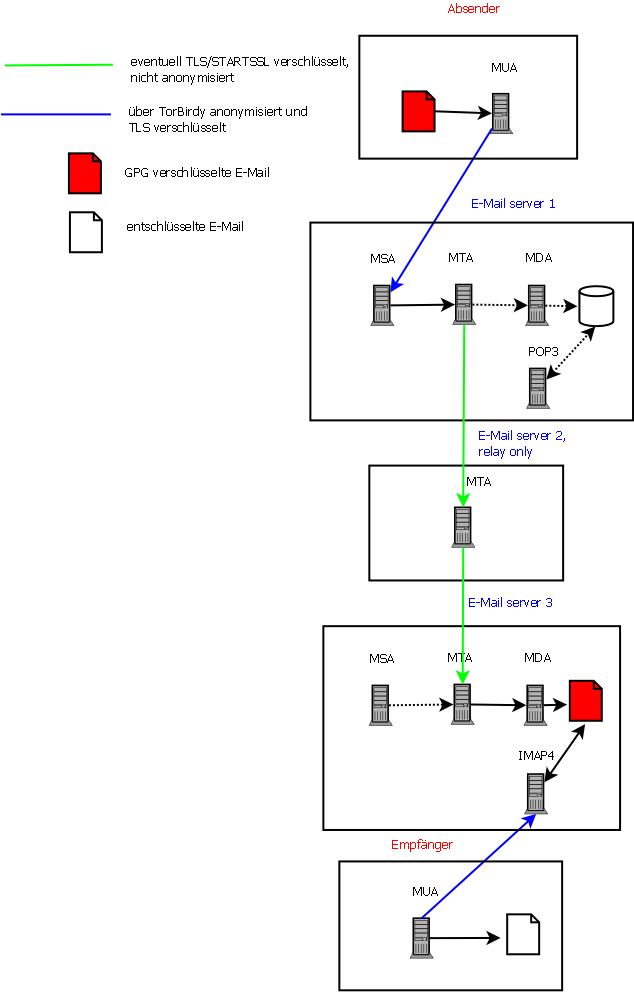
\includegraphics[scale=0.4]{Content/Problematik/BetrachtungDatenschutz/Bewertung.png}
	\caption{Übersicht Datenschutz in E-Mail Systemen}
	\label{fig:bewertung}
\end{figure}
\vfill
\clearpage


	\section{Anforderungen an eine adäquate Lösung}
		Nachfolgend werden die Anforderungen an eine adäquate Lösung formuliert. Dabei handelt es sich nicht um die Anforderungen an ein E-Mail System an sich, sondern um die Anforderungen, die relevant für größtmögliche Datensicherheit und Anonymität in einem bereits funktionierenden E-Mail System sind. Als System werden alle Komponenten bezeichnet, die beim Senden und Empfangen einer E-Mail involviert sind.

Die nachfolgenden Anforderungen sind rein funktional und beziehen sich lediglich auf Verschlüsselung und Anonymisierung.

\begin{longtable}{|c|m{12cm}|}
	\hline 
	Nummer & Anforderung \\
	\hline
	\EmptyRow 
	\hline \endhead
		\Textlabel{FA 1}{text:FA1} &
			Das System muss dem Benutzer die Möglichkeit bieten,
			den Textinhalt seiner E-Mail vor dem Versenden an den
			MSA kryptografisch zu verschlüsseln. \\
	\hline \Grayrow 
		\Textlabel{FA 2}{text:FA2} & 
			Das System muss dem Benutzer die Möglichkeit bieten,
			die Transaktion zwischen MUA und MSA über eine
			verschlüsselte Verbindung zu etablieren.\\
	\hline
		\hline
		\Textlabel{FA 3}{text:FA3} &
			Das System muss dem Benutzer die Möglichkeit bieten,
			die Verbindungsdaten der Transaktion zwischen MUA und
			MSA zu anonymisieren.\\
	\hline \Grayrow 
		\Textlabel{FA 4}{text:FA4} & 
			Das System muss dem Benutzer die Möglichkeit bieten,
			die Transaktion zwischen MUA und POP3/IMAP Server
			über eine verschlüsselte Verbindung zu etablieren.\\
	\hline
		\hline
		\Textlabel{FA 5}{text:FA5} &			
			Das System muss dem Benutzer die Möglichkeit bieten,
			die Verbindungsdaten der Transaktion zwischen MUA und
			POP3/IMAP Server zu anonymisieren.\\
	\hline \Grayrow
		\Textlabel{FA 6}{text:FA6} & 
			Das System muss dem Benutzer die Möglichkeit bieten,
			den Versand und die Zustellung der E-Mail auf MTA-Ebene
			nur über verschlüsselte Verbindungen zu erlauben.\\
	\hline
		\hline
		\Textlabel{FA 7}{text:FA7} &
			Das System muss dem Benutzer die Möglichkeit bieten,
			den Versand und die Zustellung der E-Mail auf MTA-Ebene
			nur über anonymisierte Verbindungen zu erlauben.\\
	\hline
	\CaptionLongtable{Funktionale Anforderungen}
	\label{tab:FunctionalRequirements}
\end{longtable}

Die nachfolgenden Anforderungen sind nicht funktional und beziehen sich auf mögliche Probleme, die aus der Implementierung der genannten funktionalen Anforderungen entstehen könnten.

\begin{longtable}{|c|m{12cm}|}
	\hline 
	Nummer & Anforderung \\
	\hline
	\EmptyRow 
	\hline \endhead
		\Textlabel{NFA 1}{text:NFA1} &
			Das System muss kompatibel mit den Protokollen
			SMTP, POP3 und IMAP sein.\\
	\hline \Grayrow 
		\Textlabel{NFA 2}{text:NFA2} & 
			Das System sollte die bereits existierenden Methoden
			zur Spam-Abwehr nicht erschweren. \\
	\hline
	\CaptionLongtable{Nicht-Funktionale Anforderungen}
	\label{tab:NonFunctionalRequirements}
\end{longtable}

Wie zu erkennen ist, folgt aus den funktionalen Anforderungen der Versuch, nicht nur Teile des E-Mail Verkehrs zu verschlüsseln und anonymisieren, sondern das System als ganzes. Da das betrachtete System bestehend aus den Protokollen SMTP, POP3 und IMAP aber aus verschiedenen Einzelteilen besteht, müssen die Lösungen auch spezifisch auf die jeweiligen Teilsysteme bezogen sein. Das bedeutet ebenso, dass ein direkter Bezug zu konkreten Protokollen besteht und dies keine abstrakte Anforderungsliste an irgendein E-Mail System ist.

Die nichtfunktionalen Anforderungen beschäftigen sich hingegen mit der Kompatibilität und der praktischen Einsetzbarkeit des Systems. Diese Komponenten spielen eine wichtige Rolle für eine mögliche Akzeptanz einer Lösung.

	
\chapter{Alternative Lösungen bzw. E-Mail Systeme}
	Zur Lösung der Datenschutzprobleme auf SMTP-Ebene existieren wenig wissenschaftliche Arbeiten. Eine etwas theoretische Arbeit ist \QuoteM{Untraceable Electronic Mail, Return Addresses, and Digital Pseudonyms} \RefIt{Chaum:1981:UEM:358549.358563}, welche allerdings nicht auf konkrete E-Mail Protokolle eingeht, da sie auch ca. 1 Jahr vor dem ersten SMTP Standard \RefIt{rfc821} veröffentlicht wurde.

Allerdings existieren alternative E-Mail Systeme, die das Problem des Datenschutzes auf ihre eigene Weise lösen ohne an SMTP gebunden zu sein. Dazu gehören beispielsweise Dark Mail \RefIt{Chaum:1981:UEM:358549.358563}, aber auch Bitmessage \RefIt{bitmessage}, welches auf der Bitcoin \RefIt{bitcoin} Technologie basiert.

Nachfolgend wird Dark Mail kurz besprochen.
	\section{Dark Mail}
		Als sehr genau spezifizierte Alternative zur E-Mail muss Dark Mail, bzw. \QuoteM{Dark Internet Mail Environment} \RefIt{darkmail} genannt werden. Dark Mail verwirft jegliche bekannten Protokolle wie SMTP und entwickelt ein gänzlich neues E-Mail Konzept mit den Protokollen \QuoteDirect{Dark Mail Transfer Protocol}{darkmail}{S. 82-87} und \QuoteDirect{Dark Mail Access Protocol}{darkmail}{S. 108}. Ebenso kommt ein eigenes Datenformat namens \QuoteDirect{D/MIME}{darkmail}{S. 68-81} zum Einsatz.

Auf die genauen Einzelheiten kann hier nicht eingegangen werden, da Dark Mail sehr komplex ist. Wichtig zu bemerken ist allerdings, dass es eine dem Onion Routing \RefIt{onionrouting1} \RefIt{onionrouting2} ähnliche Methodik benutzt. Ebenso kommt verschachtelte Verschlüsselung und ein durchdachtes Schlüsselsystem zum Einsatz. Allerdings ist Dark Mail auf Implementierungsebene noch nicht fertig und es existiert zum derzeitigen Zeitpunkt kein Release \RefIt{libdime}.

	\section{Bewertung}
		Nahezu alle Datenschutzmechanismen für E-Mails sind erst wesentlich später als die ursprünglichen Protokolle wie SMTP entstanden und haben sich mit der Zeit entwickelt. Viele der vorgestellten Technologien sind unabhängige Lösungen, die lediglich in Verbindung mit E-Mail Systemen verwendet werden können, andere sind wiederum Protokollerweiterungen, die sich mehr oder weniger sinnvoll in das Gesamtkonzept einfügen. Sichtbar anhand der untersuchten Technologien ist allerdings, dass hier keine konsistente Lösung vorliegt. Jede Lösung zielt auf einen anderen Bereich ab und versucht ein atomares Problem zu lösen, ohne dabei auf die Kohärenz eines in der Praxis eingesetzten E-Mail Systems achten zu können. Dies öffnet unabhängig vom Kohärenzproblem auch das Problem der Konfiguration eines konkreten Systems. Die immense Komplexität der zusammenspielenden Komponenten wurde in Kapitel 1 erhellt und ist ein praktisches Problem solcher Systeme.

Dennoch ist es möglich die genannten Systeme zu nutzen, um eine Reihe von Problemen bezüglich Datensicherheit zu lösen. Um die Inhaltsdaten des Bodies einer E-Mail für jeden außer der Empfängerperson unzugänglich zu machen, kann das asymmetrische Verschlüsselungsverfahren GPG benutzt werden. Selbst der Server-Betreiber oder ein Man-in-the-Middle ist dann nicht in der Lage, die E-Mail ohne weiteres zu entschlüsseln, unabhängig davon, in welcher Weise diese transportiert wurde. Allerdings bezieht sich GPG nur auf den Body einer E-Mail und nicht auf die Header. Ebenso ist es möglich, die Protokoll-Transaktionen von SMTP, POP3 und IMAP über direktes TLS oder STARTTLS zu verschlüsseln. Problematisch hierbei ist aber, dass eine verschlüsselte Verbindung nicht durchgängig garantiert werden kann, z.b. wenn die Verbindung über mehrere MTAs geht oder wenn der E-Mail Server erlaubt zu unverschlüsselten Verbindungen herunterzustufen, insbesondere über SMTP STARTTLS. Und letzten Endes ist eine gewisse Anonymisierung der IP-Verbindungsdaten über TorBirdy möglich. Diese gilt allerdings nur für die Kommunikation des MUA mit dem MSA bzw. POP3/IMAP server.

\autoref{fig:bewertung} zeigt sehr deutlich, dass selbst beim Einsatz all dieser Technologien und unter der Voraussetzung korrekter Konfiguration immer noch eine wesentliche Stelle nicht ausreichend anonymisiert oder verschlüsselt werden kann. Dies ist nämlich die Kommunikation zwischen mehreren MTAs. Hier kann durchgängig nicht angenommen werden, dass Transaktionen verschlüsselt sind. Ebenso sind die Verbindungen direkt und weiterleitende E-Mail Server werden über den \verb#Received# Header gekennzeichnet. Somit ist es ohne viel Aufwand möglich, den Weg, den eine E-Mail nimmt, nachzuverfolgen und zumindest die kommunizierenden E-Mail Server eindeutig zu bestimmen. Die Menge an offenen Metadaten an dieser Stelle ist so hoch, dass hier keine Gesamtlösung zu erkennen ist und u.U. Sender und Empfänger direkt identifiziert werden können.

Allerdings ist festzuhalten, dass abgesehen von der mangelnden Verschleierung der Kommunikation zwischen MTAs, die existierenden Technologien die Basis einer Gesamtlösung bilden können.

\begin{figure}[htb]
	%\Centerfloat
	\centering
	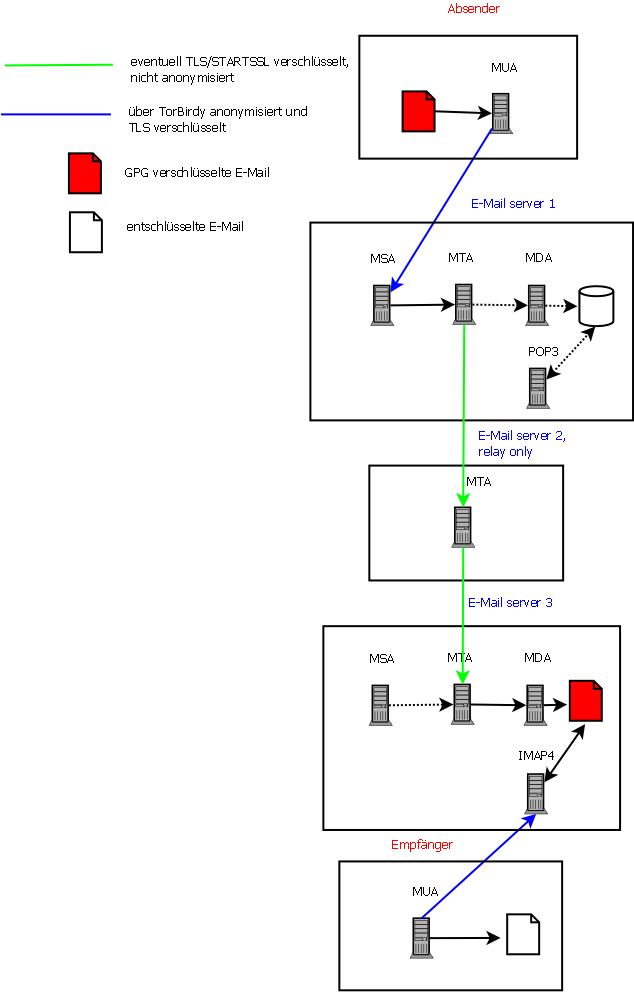
\includegraphics[scale=0.4]{Content/Problematik/BetrachtungDatenschutz/Bewertung.png}
	\caption{Übersicht Datenschutz in E-Mail Systemen}
	\label{fig:bewertung}
\end{figure}
\vfill
\clearpage


		
\chapter{Entwicklung eines SMTP-basierten Anonymisierungs-Algorithmus}
	\input{Content/Entwicklung}
	\section{Idee \& Konzept}
		Zur Lösung der Anforderungen in \autoref{tab:FunctionalRequirements} wird nachfolgend ein Algorithmus diskutiert und vorgestellt, der die Verbindung zwischen MTAs auf SMTP-Ebene anonymisieren soll, sodass Sender und Empfänger einer E-Mail nicht durch Verfolgung von IP-Adressdaten nachvollzogen werden können.

Bei der Überlegung eines solchen Algorithmus spielt vor allem \autoref{text:NFA1} eine Rolle. Alternative E-Mail Systeme mit einem Schwerpunkt auf Datensicherheit wurden bereits in Kapitel 3 vorgestellt. Im Zuge dieser Arbeit wird allerdings versucht, der Akzeptanz halber eine SMTP-basierte Lösung zu entwickeln. Dies soll, mit minimalem Aufwand für E-Mail Server Betreiber und Nutzer, eine Verbesserung der Datensicherheit ermöglichen.

Bei der Wahl und Entwicklung des Algorithmus wurde vor allem Wert darauf gelegt, dass keine spezifischen SMTP Erweiterungen notwendig sind. Somit soll dieser auf dem Minimum des IMF und SMTP Protokolls fußen.

Die Anonymisierung soll über zufälliges Routing realisiert werden, welches kryptografisch gestützt wird. Alle Informationen zum Routing sollen in der E-Mail kodiert sein. Jeder Knoten soll zu jedem Zeitpunkt nur den Nachfolger und Vorgänger kennen. Die originale E-Mail darf nicht modifiziert werden, was bedeutet, dass ein Verschachtelungsverfahren angewendet werden muss.


		\subsection{Algorithmus}
			Der Algorithmus wird nachfolgend \QuoteM{MystMail Algorithmus} genannt und ist vom Grundprinzip dem Onion Routing \RefIt{onionrouting2} nicht unähnlich.

Der Algorithmus bezieht sich allerdings nicht nur auf MTAs, sondern muss auch auf der Ebene der Kommunikation zwischen MUA und MSA eingreifen.

In ihrer Funktionsweise ist die MystMail eine gewöhnliche E-Mail, die eine Art Liste von Relay Servern beinhaltet. Die E-Mail wird also nicht direkt an den schlussendlichen Empfänger gesendet, sondern über mehrere Relay Server (auch \QuoteM{Hops} genannt) geleitet, basierend auf den kodierten Informationen in der E-Mail. Dies ist der Anonymisierungspfad. Damit dieser Pfad selbst weder für die Hops noch für irgendjemand sonst sichtbar ist, muss er kryptografisch in die E-Mail eingebettet werden.

Die sogenannte Liste von Hops ist also keine Liste, die in Form von Klartext als Header festgesetzt wird. Stattdessen wird die originale E-Mail inklusive Header über ein asymmetrisches Verschlüsselungsverfahren mit dem öffentlichen Schlüssel des ersten Hops verschlüsselt und fungiert jetzt als Body einer neuen E-Mail, die an denselben Hop gerichtet ist, gewissermaßen die erste MystMail. Für den nächsten Hop wird das Verfahren mit der soeben neu erstellten MystMail wiederholt. Dies kann theoretisch beliebig oft wiederholt werden und hat zur Folge, dass eine verschachtelte Verschlüsselung vorliegt, jede Schicht mit einem anderen öffentlichen Schlüssel verschlüsselt. Dies bedeutet wiederum, dass kein Hop in der Mitte des Pfades an die übernächste MystMail gelangen kann, da er nicht den privaten Schlüssel dafür besitzt. Somit kennt jeder Hop nur Vor -und Nachfolgehop.

Ist nun die schlussendliche MystMail mit der impliziten Liste von Hops vollständig durch den MUA erstellt, wird sie an den ersten Hop gesendet. Dieser entschlüsselt den Body mit seinem privaten Schlüssel und erhält die nächste MystMail mit Informationen zum nächsten Hop im \verb#To:# Headerfeld. Diese MystMail versendet er über SMTP nun an den nächsten Hop, welcher die nächste MystMail entschlüsselt, usw. Die MystMail hat jedoch ein dediziertes Headerfeld \verb#X-Myst-Mail: 1#, der SMTP-kompatibel markiert, dass diese E-Mail eine spezielle E-Mail ist. Durch den ganzen Pfad ist dieses Headerfeld aktiv. Gelangt die E-Mail an den schlussendlichen Empfänger, so entschlüsselt dieser den Body der E-Mail ohne bereits zu wissen, dass er der Empfänger ist. Erst nachdem der MTA keinen \verb#X-Myst-Mail: 1# findet, weiß er, dass er der schlussendliche Empfänger ist und kann die entschlüsselte E-Mail lokal über den MDA zustellen.

Dieser Algorithmus wird auf MTA-Ebene durch das \verb#X-Myst-Mail: 1# Headerfeld ausgelöst. Ist dieses nicht Bestandteil des Headers, so wird die E-Mail nach den gewöhnlichen Regeln des MTAs zugestellt oder weitergeleitet. Die Art und Weise, wie dieser Algorithmus auf MUA Ebene ausgelöst wird, ist nicht spezifiziert.

Sowohl der Verschlüsselungsalgorithmus für die verschachtelten E-Mails als auch der Zufallsalgorithmus zur Auswahl der Hops wird hier nicht spezifiziert.

In chronologischen Schritten kann der Algorithmus folgendermaßen dargestellt werden:\\

\begin{minipage}{\linewidth}
\begin{mail}{MystMail-Algorithmus Simulation}{MystMail-Algorithmus}
MUA (Sender): empfängt Liste von Hops von einem zentralen
              Server
MUA (Sender): wählt aus der Liste einen zufälligen Pfad aus
MUA (Sender): erstellt die initiale verschachtelte MystMail
              für den ersten Hop
MUA (Sender): reicht die MystMail an seinen MSA ein
MSA (Sender): nimmt MystMail entgegen
MTA (Sender): sendet die MystMail an den ersten Hop
MTA (1. hop): nimmt die MystMail entgegen
MTA (1. hop): erkennt den "X-Myst-Mail: 1" Header
MTA (1. hop): entschlüsselt den Body der E-Mail mit seinem
              öffentlichen Schlüssel
MTA (1. hop): erkennt, dass auch dort ein "X-Myst-Mail: 1"
              Header vorliegt
MTA (1. hop): benutzt den entschlüsselten Text als neue E-Mail
              und sendet die MystMail an die Adresse aus dem
              "To:" Headerfeld, den 2. Hop
MTA (2. hop): nimmt die MystMail entgegen
[...] (wie 1. hop)
MTA (3. hop): nimmt die MystMail entgegen
[...] (wie 1. hop)
MTA (Empfänger): nimmt die MystMail entgegen
MTA (Empfänger): erkennt das "X-Myst-Mail: 1" Headerfeld
MTA (Empfänger): entschlüsselt den Body der E-Mail mit seinem
                 öffentlichen Schlüssel
MTA (Empfänger): erkennt, dass im entschlüsselten Text kein
                 "X-Myst-Mail: 1" Headerfeld vorliegt
MTA (Empfänger): leitet die E-Mail an den MDA weiter
MDA (Empfänger): stellt lokal zu
MUA (Empfänger): ruft E-Mail vom POP3/IMAP Server ab
                 und sieht die original E-Mail
                 mit dem korrekten "From:" Feld vom Empfänger
\end{mail}
\end{minipage}

Auf Basis des MTA ist also eine Entscheidung notwendig, abhängig vom \verb#X-Myst-Mail# Headerfeld. Diese Entscheidung kann folgendermaßen dargestellt werden:\\
\\
\begin{minipage}{\linewidth}
\begin{mail}{MystMail MTA Entscheider}{mtadecider}
// either relays a MystMail or delivers the inputmail in case
// it is not a MystMail
function processMail (inputmail) {
  header = inputmail.header;
  body = inputmail.body;
  if header.getField("X-Myst-Mail").notNull()
    newMystMail = decrypt(body);
    envelope = createEnvelope(newMystMail);
    send(newEnvelope);
  else
    deliverToMDA(inputmail);
}

// creates the Envelope that carries Meta-Data for the
// SMTP transaction, such as "RCPT TO" and "MAIL FROM"
function createEnvelope(inputmail) -> Envelope {
  from = inputmail.header.getField("From");
  to = inputmail.header.getField("To");
  
  return new Envelope(mail = inputmail
                     , RCTP = [to]
                     , MAILFROM = from);
}
\end{mail}
\end{minipage}

Für den MUA liegt folgendes Verhalten vor:\\

\begin{minipage}{\linewidth}
\begin{mail}{MystMail-Erstellung (MUA)}{mysterstellung}
// creates the initial MystMail
function createMystMail(inputmail) -> EMail {
  hops = getHopList();
  path = chooseHopPath(hops) ++ inputmail.recipient;
  newmail = inputmail;
  
  for hop in path {Alle Informationen zum routing sollen in der E-Mail kodiert sein.
  	if (hop == path[0])
  	  from = "myst@" ++ inputmail.sender.address.domain;
  	else  
  	  from = hop.prev.address;
  	to = "myst@" ++ hop.domain;
    body = encrypt(hop, newmail);
    newmail = EMail(From = from
                   , To = to
                   ).addHeader("X-Myst-Mail: 1");
  }

  return newmail;
}
\end{mail}
\end{minipage}


\autoref{fig:algorithmus} zeigt schematisch den Ablauf des Algorithmus. Die initiale E-Mail ist 4-fach verschachtelt verschlüsselt und geht über 3 Hops. Jeder Hop entschlüsselt den Body der eingegangenen E-Mail, benutzt diesen entschlüsselten Text als vollständige IMF-kompatible E-Mail inklusive Header und Body und leitet diese dann an den nächsten Hop weiter. Der Empfänger MTA erkennt, dass kein \verb#X-Myst-Mail# Headerfeld vorliegt und reicht die unveränderte originale E-Mail an den MDA weiter. Die farbig markierten Pfeile zeigen an, welcher Teil der MystMail gerade weitergesendet wird.

Anzumerken ist hierbei, dass abgesehen von der originalen E-Mail alle Header das \verb#From# und \verb#To# Feld verschleiern, indem der Benutzername \verb#myst# verwendet wird. Technisch gesehen ist es unerheblich, wie der Benutzername definiert ist, da dies das Verhalten des MystMail MTAs nicht verändert.

\begin{figure}[htb]
	%\Centerfloat
	\centering
	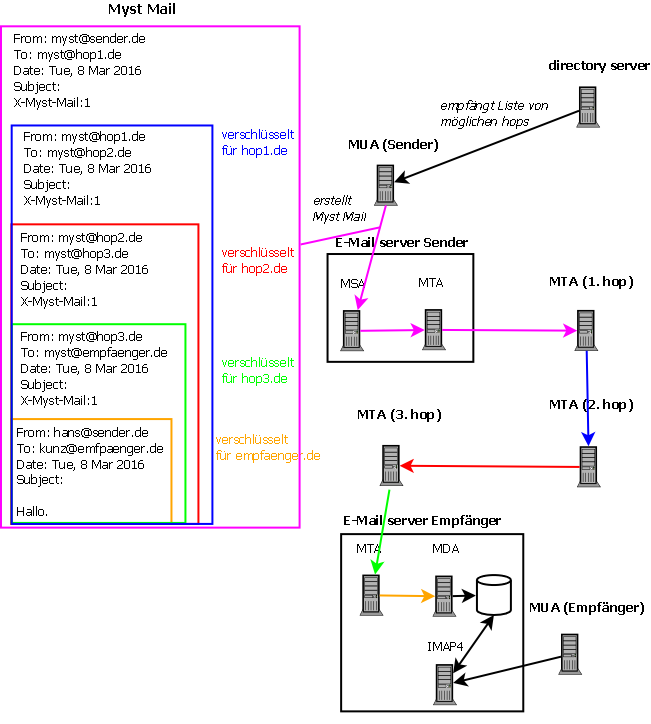
\includegraphics[scale=0.5]{Content/Entwicklung/IdeaConcept/Algorithmus.png}
	\caption{Übersicht MystMail Algorithmus}
	\label{fig:algorithmus}
\end{figure}
\vfill
\clearpage
	\section{Methoden}
		Die hier beschriebenen Methoden beziehen sich auf die wissenschaftliche Arbeitsweise, sowohl auf theoretischer als auch auf praktischer Ebene, welche in dieser Arbeit Anwendung findet.

Dem Geiste nach wird versucht dem wissenschaftstheoretischen Ideal aus der \QuoteM{Logik der Forschung} \RefIt{popper1998karl} von Karl R. Popper zu entsprechen. Demnach ist die Arbeit als Ganzes vor allem ein Diskussionsvorschlag an den wissenschaftlichen Apparat. Sie stellt aber ebenso eine Behauptung auf mit der Erwartung, dass an derselben Falsifikationsversuche durchgeführt werden können.

Das Wesen der Falsifikation ist hier allerdings etwas anders als in klassischen empirischen Wissenschaften wie der Physik. Neben der logischen Falsifikation, die sich vor allem auf Argumentationsfehler und Logikfehler im Allgemeinen bezieht, ist die sogenannte empirische Falsifikation im Kontext der hier aufgestellten Behauptungen weniger exakt und die Trennung beider Formen weniger eindeutig. Konzeptionelle Fehler und Schwächen können sowohl a priori, als auch a posteriori erkannt werden, da die Tauglichkeit des vorgeschlagenen Systems nicht rein formal bestimmt werden kann. Viele in der Praxis relevante Details und Faktoren wirken auf das System als ganzes ein und machen Falsifikationsversuche schwieriger. Mögliche Angriffsvektoren werden häufig erst entwickelt oder entdeckt, wenn ein System bereits eine Weile in Benutzung ist. Gerade deshalb sind weite Teile des vorgeschlagenen Systems nur sehr abstrakt beschrieben. Somit konzentriert sich diese Arbeit mehr auf eine Idee, weniger auf ein vollständig durchdachtes Konzept und kann letzteres auch nicht leisten.

Die genannte Idee wird im Zuge dessen argumentativ unterstützt, sowohl im Rückblick auf das existierende E-Mail System und seine Schwächen, als auch im Hinblick auf Systeme im allgemeinen, die ähnliche algorithmische Methoden erfolgreich verwenden.

Auf dieser Basis wird weiterhin versucht nachzuweisen, dass der Algorithmus im Kern implementierbar ist und die Proof of Concept Implementierung zumindest die wichtigsten Anforderungen aus \autoref{tab:FunctionalRequirements} und \autoref{tab:NonFunctionalRequirements} tatsächlich erfüllen kann.

Die Implementierung wird sich auf den Kern-Algorithmus beschränken und ein minimales Testsystem zur Simulation von MTA-Kommunikation beinhalten.

Bei der Entwicklung der Implementierung wird eine abgewandelte Form des Prototyping Modells \RefIt{swprototyping} angewendet. Dabei ist der erste Schritt die Entwicklung eines Testsystems, das ein verteiltes System simulieren kann. Andernfalls ist es schwierig, in kurzen Abständen Codeänderungen durchzuführen und deren Auswirkungen zu überprüfen. Sobald dieses Testsystem steht, wird eine existierende SMTP Implementierung ausgewählt und diese ins Testsystem integriert. Das Testsystem beschränkt sich hierbei auf sichtbare Laufzeittests. Ist diese grundlegende Funktionalität gegeben, so wird der eigentliche Algorithmus injiziert und ohne weitere Iterationen vervollständigt. Erst nach dieser Phase findet eine Reflexion statt, die Refactoring oder sogar eine vollständige Neuentwicklung zur Folge haben kann. Der Dokumentationsprozess ist ein fortlaufender Prozess, der in jeder Phase der Entwicklung stattfindet.



	\section{Realisierung}
		Die Realisierung auf Basis des Prototyping Modells durchläuft mehrere Phasen. Zunächst wird ein Testsystem entwickelt, das auf Docker \RefIt{dockerhp} basiert. Dieses Testsystem wird es erlauben, mehrere MTAs miteinander isoliert kommunizieren zu lassen. Dafür muss ebenso eine SMTP Implementierung gewählt werden. Nach der Entwicklung des Testsystems wird der Einsprungpunkt gesucht, an dem der Algorithmus in das bestehende SMTP Protokoll injiziert werden kann. Ist dieser gefunden, wird zunächst der MystMail MTA Entscheider (Code \ref{mtadecider}) implementiert. Dieser wird noch nicht die Logik für das Erstellen der weiterzuleitenden MystMail beinhalten oder das Weiterleiten selbst, sondern lediglich die Entscheidungslogik testen. Danach kann überprüft werden, ob das SMTP Protokoll immer noch einwandfrei funktioniert und beim Erkennen einer MystMail der entsprechende Entscheidungszweig erreicht wird. Ist die Korrektheit hier verifiziert, wird der Teil des MystMail MTA Entscheiders implementiert, der die Nachricht, zunächst noch unverändert, an einen vordefinierten MTA weiterleitet. Somit wird das Weiterleiten zwischen den MTAs getestet. Ist das Weiterleiten möglich, so wird die eigentliche Logik zum Entpacken einer MystMail implementiert, inklusive dem Interpretieren des Bodies und dem Erstellen eines Envelope. Nach diesem Schritt wird eine statische initiale MystMail per Hand erstellt und das Entpacken sowie die Weiterleitung zwischen den MTAs getestet. Als letzter Schritt wird die MystMail-Erstellung (Code \ref{mysterstellung}) als SMTP-Gateway implementiert, nicht als MUA Erweiterung. Dies geschieht aus Gründen der Einfachheit.

Nachfolgend werden die einzelnen Phasen der Entwicklung beschrieben, Entscheidungen erklärt und Probleme erläutert.

\label{section:realisierung}
	
		\subsection{Testsystem}
			Für das Testsystem wird eine isolierte Umgebung benötigt, die ausreichend Kontrolle über Netzwerkdetails erlaubt und trotzdem möglichst frei von etwaigen Netzwerkproblemen ist. Würde hier echte Hardware eingesetzt werden, so käme das Problem hinzu, dass auf Hardware-Ebene Probleme und Fehler das System beeinträchtigen könnten. Eine manuelle lokale Konfiguration innerhalb eines Host-Systems, die das simulieren mehrerer MTAs erlaubt, ist aufgrund der Konfigurationskomplexität ebenso unerwünscht. Ebenso würde dies eine Abhängigkeit vom Host-System und dessen Konfiguration bedeuten. Aus diesem Grund wird eine Container-Software eingesetzt, die die entsprechenden Abstraktionsschichten bereits bereitstellt. Sie erlaubt mehrere gleichartige Prozesse isoliert laufen zu lassen und dieselben über eine definierte softwareseitige Netzwerkschnittstelle kommunizieren zu lassen. Für diese Art von Software existieren mehrere Lösungen. Für die Realisierung wird hier allerdings die Software \QuoteM{Docker} \RefIt{dockerhp} eingesetzt.

Docker ist keine Hardwarevirtualisierung. Es ist eine Abstraktionsschicht, die es erlaubt Prozesse in isolierten User-Spaces auf demselben Betriebssystemkernel laufen zu lassen. Dazu benutzt es Kernel Features wie Cgroups und Kernel Namespaces. Auf Dateisystem-Ebene wird UnionFS benutzt.

Die praktische Funktionsweise reduziert sich auf folgenden Ablauf: Der Benutzer erstellt eine Definitionsdatei mit dem Namen \QuoteM{Dockerfile}. Diese definiert gewissermaßen den Installationsprozess eines vollständigen Betriebssystems, der darin benötigten Applikationen, sowie die Art und Weise wie diese ausgeführt und konfiguriert werden. Auf Basis dieses Dockerfiles kann ein \QuoteM{Docker Image} erstellt werden. Ein Docker Image kann als Vorlage betrachtet werden, mit der eine Chroot-ähnliche Umgebung erstellt und ausgeführt werden kann. Diese ausgeführte Umgebung wird \QuoteM{Docker Container} genannt. Wichtig ist dabei, zu wissen, dass das Image aus mehreren UnionFS-Layern besteht (pro Dockerfile-Anweisung ein Layer). Wenn ein Container gestartet wird, so wird auf die Daten aus dem Image zugegriffen. Allerdings sind diese immer read-only. Sobald Änderungen an Dateien innerhalb eines Containers gemacht werden, wird die read-only Schicht des Images mit einer read-write Schicht des laufenden Containers zusammengeführt, ohne dass die Daten des Images sich dabei verändern. Somit können auf Basis eines beispielsweise gemeinsamen MySQL-Images mehrere MySQL-Instanzen gestartet werden, die alle dieselbe Version, dasselbe Betriebssystem und dieselbe Umgebung besitzen, aber dennoch voneinander isoliert sind, sowohl auf Prozess-, Netzwerk- und Dateisystem-Ebene. Beim Starten von Containern ist es allerdings möglich, diese miteinander zu verbinden, so dass sie auf Netzwerkebene miteinander kommunizieren können.

Mithilfe dieses Systems wird es möglich, mehrere gleiche MTAs zu starten und zu verbinden. Dabei können diese sich dennoch in der Konfiguration unterscheiden, da im laufenden Container Änderungen vorgenommen werden können. Ebenso ist es möglich, über Umgebungsvariablen oder Mountpoints, die vom Host in den Container zeigen, den Zustand und die Konfiguration eines Containers zu steuern. Ebenso sind die Container nahezu vollständig unabhängig vom laufenden Host-System, da ein Container bereits ein vollständiges Betriebssystem darstellt und lediglich mit dem Kernel des Host-Systems über den Docker Daemon kommuniziert wird.

Es werden gemäß \autoref{fig:algorithmus} also 5 E-Mail Container gestartet. Alle 3 Hops und der E-Mail Server des Empfängers haben dieselbe Konfiguration. Nur der E-Mail Server des Senders hat eine abweichende Konfiguration, da dieser als SMTP Gateway fungiert und anstelle des MUAs die initiale MystMail generiert. Alle Container werden in einem Netzwerk zusammengefasst und können untereinander kommunizieren.

Dieses System erlaubt es nun, fortlaufend Laufzeittests durchzuführen. Diese finden nicht automatisiert statt, sondern werden über die laufenden Prozesse in den Containern und deren Logdateien manuell durchgeführt.

Die Implementierung des Testsysems ist im Anhang einsehbar.

		\subsection{Implementierung}
			Nicht gerade ein Problem dieser Arbeit, aber ein Problem für eine mögliche praktische Benutzung ist das Fehlen einer professionellen Implementierung. Diese ist aber nicht sinnvoll ohne eine konkrete Spezifikation wie auf Seite \pageref{section:spezifikation} genannt möglich.

Die hier präsentierte Implementierung ist eine Proof-of-Concept Implementierung und in keiner Weise für den Einsatz gedacht. Unschöner Weise hängt sie sogar von interner API ab.
Eine professionelle Implementierung würde hingegen als strenges Modul bzw. Plugin entwickelt werden müssen. Darüber hinaus müssen weitere wichtige Gesichtspunkte berücksichtigt werden wie die Wahl der zugrundeliegenden SMTP Implementierung und Sprache.

Dieser Punkt beinhaltet implizit einige der nachfolgend noch genannten Probleme.
			\subsubsection{Wahl der SMTP-Software}
				Bei der Wahl der SMTP-Software waren mehrere Gesichtspunkte von besonderer Bedeutung:
\begin{itemize}
\item wird die Software tatsächlich eingesetzt?
\item wird die Software aktiv entwickelt und gepflegt?
\item in welcher Sprache ist die Software geschrieben?
\item ist die Software (ausreichend) dokumentiert?
\item wie kompliziert ist die Konfiguration?
\item wie einfach lässt sich die innere Logik verändern?
\end{itemize}

Diese Punkte sind wichtig, um eine mögliche Weiterentwicklung der Idee auf Basis derselben Implementierung einfacher zu machen, obwohl diese nur eine Proof-of-Concept Implementierung ist. Ebenso vereinfachen sie die Implementierung an sich und machen diese einfacher zu verstehen. Einige der Punkte sind auch relevant für Sicherheitsbedenken. Dies betrifft vor allem die Programmiersprache und die Komplexität der inneren Logik.

Zur näheren Auswahl kamen aufgrund der genannten Gesichtspunkte folgende SMTP-Softwarelösungen:
\begin{enumerate}
\item Sendmail \RefIt{sendmailhp}
\item OpenSMTPD \RefIt{opensmtpdhp}
\item Haraka \RefIt{harakahp}
\end{enumerate}

Sendmail kam in die nähere Auswahl, da es eine sehr alte Lösung ist, die extrem hohe Verbreitung hat. Ebenso ist der Code in weiten Teilen sehr gut dokumentiert. Allerdings ist die Konfigurationskomplexität äußerst hoch und der Code beinhaltet viel Indirektion, da der Code über die Zeit gewachsen ist. Sendmail ist in C geschrieben.

Als Alternative zu Sendmail fiel der Blick auf OpenSMTPD, dessen erstes stabiles Release aus dem ersten Quartal 2013 stammt \RefIt{opensmtpdrel}. Dies versprach eine bessere Strukturierung des Codes als Sendmail. Allerdings musste festgestellt werden, dass so gut wie keine Dokumentation auf Code-Ebene vorhanden ist. OpenSMTPD ist ebenfalls in C geschrieben. Aufgrund der mangelhaften Dokumentation schied dies also Option aus.

Als weitere Alternative wurde Haraka betrachtet. Haraka ist ein SMTP Server, welcher in Node.js geschrieben ist, also praktisch in Javascript. Dies öffnete einige Bedenken, da Javascript schwach und dynamisch typisiert ist und diverse Details des SMTP-Protokolls auf sehr exaktem Verhalten bezüglich der Bit-Länge gesendeter Nachrichten beruhen. Allerdings besitzt Haraka ein Plugin-System, welches auf Callbacks bzw. Hooks basiert, die es dem Programmierer erlauben, an unterschiedlichen Stellen in der Verarbeitung einer Transaktion anzusetzen und diese zu überschreiben oder lediglich zusätzliche Logik zu definieren. So ist es beispielsweise möglich, zu definieren was der Haraka Server nach einem empfangenen \verb#DATA# SMTP-Kommando tut, ohne bereits bestehenden Code verändern zu müssen. Ebenso ist die Dokumentation in weiten Teilen ausreichend, weshalb diese SMTP-Softwarelösung trotz der Bedenken über die Schwächen des Javascript-Typsystems als Basis der Implementierung ausgewählt wurde.

			\subsubsection{Übersicht über Haraka}
				Wie bereits erwähnt, basiert Haraka auf einem explizit entwickelten Plugin-System. Weite Teile der Kernfunktionalität von Haraka sind über das Plugin-System selbst implementiert und werden als Standard-Plugins mitgeliefert. Diese können dann über diverse Konfigurationsdateien im Ordner \verb#config# direkt gesteuert werden. Ebenso kann definiert werden, welche Plugins überhaupt ausgeführt werden und in welcher Reihenfolge. Dies ist der Kern der Haraka-Konfiguration und befindet sich in der Datei \verb#config/plugins# im Basisordner.

Interessante hooks, die für die Implementierung von Bedeutung sind oder sein können, sind die folgenden:
\begin{itemize}
\item \verb#connect_init#: wird beim Start einer Verbindung aufgerufen
\item \verb|lookup_rdns|: liefert den reverse DNS
\item \verb#connect#: wird nach \verb|lookup_rdns| aufgerufen
\item \verb#mail#: hier können die Absender examiniert werden
\item \verb#rcpt#: hier können die Rezipienten examiniert werden
\item \verb#data#: wird beim \verb#DATA# SMTP Kommando aufgerufen
\item \verb#data_post#: wird am Ende des \verb#DATA# Kommandos aufgerufen, wenn der Client mit einem Punkt in einer Zeile signalisiert, dass die E-Mail Daten vollständig sind und der Server antworten kann
\item \verb#queue#: bevor die Mail in die Queue gelangt
\item \verb#get_mx#: wird beim Versenden aufgerufen, um den MX Record des empfangenden MTAs festzustellen
\end{itemize}

Das Plugin-Konzept sieht vor, dass mehrere Plugins denselben Hook verwenden können. Dafür muss am Ende der Funktion ein entsprechender Return Code zurückgegeben werden.

Um ein Open Relay zu definieren, kann man beispielsweise beim \verb#rcpt# Hook ansetzen, und ,abhängig von diversen Regeln, eine Weiterleitung erlauben oder nicht:
\begin{JavaScript}{Haraka Relay}{hrelay}
/**
 * This relays the mssage if is_valid_rcpt(recipient) returns true
 */
exports.hook_rcpt = function(next, connection, params) {
	// check if the recipient is valid (e.g. in a list)
	if (is_valid_rcpt(params[0]) == true) {
		connection.relaying = true;
	}
	return next(OK); // no further plugins on this hook will run
}
\end{JavaScript}

Wie hier zu sehen ist, existieren in Haraka einige grundsätzliche Objekte, die etwaige Informationen tragen. Auf der äußersten API Schicht befindet sich das \QuoteM{Connection Object} (\verb#connection# auf Code-Ebene). Dies wird für jede Verbindung, die Haraka mit einem anderen MTA eingeht erstellt und hat eine eindeutige UUID. Es trägt allgemeine Informationen über den Remote Server. Ebenso stellt es allerdings die Verbindung zur nächsten API-Schicht her, der Transaktion. \verb#connection.transaction# ist ein Objekt, das die gerade ablaufende Transaktion beschreibt. Es ist erst valide, nachdem \verb#MAIL FROM# gesendet wurde und wird beim Erreichen der Mail-Queue vernichtet wenn \verb#RSET# gesendet wird oder wenn \verb#MAIL FROM# nicht akzeptiert wurde. Innerhalb des Transaktions-Objekts sind weitere Objekte gekapselt, die die Informationen über den eigentlichen Vorgang enthalten. Das Transaktions-Objekt ist im Grunde der Umschlag der E-Mail. Es enthält die SMTP Informationen über Empfänger in \verb#transaction.rcpt_to# und Sender in \verb#transaction.mail_from#, ebenso wie die E-Mail selbst über die Objekte \verb#transaction.header# (alle Headerfelder) und \verb#transaction.body# (Text der E-Mail). Hierüber ist es möglich, an alle Informationen während einer SMTP-Sitzung zu gelangen, diese zu manipulieren oder abhängig von den Daten (z.B. Existenz von Headerfeldern) weitere Logik ausführen zu lassen. Weiterhin existiert ein ein \QuoteM{Outbound Modul}, welches über das Objekt \verb#outobund# ansprechbar ist. Über dieses Objekt ist es möglich, explizit E-Mails zu verschicken, beispielsweise wenn ein Plugin während der Verarbeitung selbst eine neue E-Mail schicken möchte.
Als letztes interessantes Objekt existiert im Connection Objekt das Objekt \verb#connection.results#, welches dazu benutzt werden kann Zustände und Informationen zu speichern, die dann über mehrere Plugins hinaus abrufbar sind (z.B. logs).

			\subsubsection{Wahl des Einsprungpunktes}
				Für die Wahl des Einsprungpunktes kamen mehrere Ansätze in die nähere Auswahl.

Der erste Ansatz war die E-Mails kurz bevor sie die Queue erreichen, im Hook \verb#queue# abzufangen und die E-Mail manuell weiterzuleiten, beispielsweise indem über \verb#outbound.send_email(...)# eine neue E-Mail erstellt und versendet wird. Das Problem hierbei ist allerdings, dass der \verb#queue# Hook speziell ist und man diesen nur vollständig überschreiben kann, nicht aber nur zusätzliche Logik einführen kann. Dies erhöht den Implementierungsaufwand.

Eine weitere Möglichkeit wäre gewesen, an mehreren Stellen anzusetzen, beispielsweise bei den Hooks \verb#mail# und \verb#rcpt#, und für jede Station Informationen zu sammeln, diese dann im \verb#connection.results# Objekt zu speichern und dann zu einem späteren Zeitpunkt eine neue E-Mail zu versenden oder die bestehende zu manipulieren. Da dies allerdings erhöhter Aufwand ist und einen globalen Zustand beinhaltet, wurde diese Idee verworfen.

Der letzte Ansatz war, im Hook \verb#data_post# anzusetzen, direkt nachdem die E-Mail Daten eingegangen sind, also das SMTP Kommando \verb#DATA# abgeschlossen ist. Dies hat mehrere Vorteile. Zum einen kann dieser Hook durch andere Plugins normal weiterverarbeitet werden und zum anderen erlaubt er an dieser Stelle das Transaktionsobjekt, welches gerade erstellt wurde, ohne viel Seiteneffekte direkt zu manipulieren. Ebenso ist dies eine zentrale Stelle, an der noch relativ wenig Plugin-Logik ausgeführt worden ist, sodass kein kompliziertes Speichern von Zwischendaten erforderlich ist.

Somit fiel die Wahl auf den letzten Ansatz und hatte folgende Implikationen:
\begin{itemize}
\item Einsprungpunkt nachdem das SMTP Kommando \verb#DATA# vollständig ausgeführt wurde (nach dem E-Mail Text)
\item keine Zwischenzustände nötig
\item erlaubt das Weiterverarbeiten durch andere Plugins
\item direktes Modifizieren des Transaktionsobjektes: E-Mail und andere Meta-Daten werden direkt manipuliert
\end{itemize}
				
	
			\subsubsection{Implementierung MTA-Entscheider}
				Nachfolgend wird der Hauptteil des Implementierungscodes aufgezeigt, allerdings ohne die Hilfsfunktionen. Dies soll eine Übersicht über den Haraka-spezifischen Algorithmus für den MTA-Entscheider geben.

\begin{minipage}{\linewidth}
\begin{JavaScript}{Haraka MTA-Entscheider}{hentscheider}
exports.hook_data_post = function(next, connection) {
    // if we have a myst mail, we need to inject our Protocol
    if (is_myst_mail(connection.transaction.header)) {
        // we decrypt the mail body and treat it as raw
        // mail data
        var decrypted_email = myst_decrypt(connection.
        	transaction.body.bodytext);

        // replace the current transaction object
        var t = transform_transaction(decrypted_email,
        	connection);
        connection.transaction = t;

        // the unpacked mail is a myst mail too, 
        // relay it
        if (is_myst_mail(connection.transaction.header)) {
            connection.relaying = true;
        }
    }

    // let the other handlers do what they want, we are
    // finished injecting our logic, the rest is still
    // SMTP compliant
    next();
}
\end{JavaScript}
\end{minipage}

Die Funktionen \verb#myst_decrypt()# und \verb#transform_transaction()# können zunächst leere Funktionen sein. Wichtig ist hier lediglich die Funktion \verb#is_myst_mail()#, welche folgendermaßen definiert ist:

\begin{JavaScript}{Haraka Myst header checker}{hismystmail}
function is_myst_mail(header) {
    if (header.get("X-Myst")) {
        return true;
    }

    return false;
}
\end{JavaScript}

Damit ist der erste Teil des MTA-Entscheider bereits implementiert und die Logik für das Entpacken und Erstellen der neuen E-Mail kann implementiert werden.

Die Verschlüsselung und Entschlüsselung ist hier lediglich Base64. Die Funktion \verb#transform_transaction()# wird aufgrund ihrer Komplexität nur im Anhang gezeigt, % toref
da sie ebenso auf interner Haraka-API aufbaut.

Ebenso wichtig ist, anzumerken, dass \verb#connection.relaying = true;# im MTA-Entscheider bedeutet, dass der MTA für alle MystMails ein Open Relay ist. Deshalb kann und sollte ab Zeile 16 weitere Logik darüber entscheiden (z.B. eine Whitelist), ob die E-Mail weitergeleitet werden darf.

			\subsubsection{SMTP-Gateway und MystMail Erstellung}
				Um die initiale MystMail zu erstellen, die die Informationen über die Hops verschlüsselt in sich trägt, wird diese der Einfachheit halber im MSA, also gewissermaßen einem SMTP-Gateway, generiert.

Die Liste der Hops ist statisch und vordefiniert für Testzwecke. Es liegt somit kein Zufallsalgorithmus vor. Die Verschlüsselung ist ebenso lediglich Pseudoverschlüsselung und kodiert gemäß Base64.

\begin{minipage}{\linewidth}
\begin{JavaScript}{Haraka Myst Erstellung}{hcreatemystmail}
function create_myst_mail(transaction) {
	// recipient is always the last hop
	var recipient = transaction.rcpt_to[0].host;
	var hops = get_hops();
	hops.push(recipient);

	// innermost mail, untouched
	var old_mail = get_raw_mail(transaction.body);

	var i;
	var new_mail = old_mail;
	for (i = hops.length - 1; i >= 0; i--) {
		if (i == 0) {
			// first hop, "from" must be the actual sender
			var sender = transaction.mail_from.host;
			new_mail = create_mail_for_hop(sender, hops[i],
			             date, new_mail);
		} else {
			new_mail = create_mail_for_hop(hops[i-1],
			             hops[i], date, new_mail);
		}
	}

	return new_mail;
}
\end{JavaScript}
\end{minipage}

Die Hilfsfunktionen lassen sich im Anhang einsehen. % toref

Nachdem die Mail erstellt ist, wird ähnlich wie beim MTA-Entscheider im Hook \verb#data_post# angesetzt und das Transaktions-Objekt manipuliert, um die dort enthaltene E-Mail mit der MystMail auszutauschen. Der entsprechende Code ist etwas kompliziert und ebenfalls im Anhang einsehbar.
 
			\subsubsection{Haraka Konfiguration}
				Nun müssen die Implementierungen noch adäquat in das Plugin-System integriert werden. Haraka Plugins werden erst ausgeführt, wenn sie in der Konfigurationsdatei \verb#config/plugins# in der korrekten Reihenfolge aufgelistet sind. Ebenso müssen einige weitere Anpassungen gemacht werden, damit ein Testlauf möglich wird. Beispielsweise muss der \verb#get_mx# Hook überschrieben werden, da hier nur lokale Systeme ohne MX-Record vorliegen. Die Implementierung ist ebenso im Anhang einsehbar. % toref

Die Konfigurationsdatei für die Hops ist folgendermaßen definiert:
\begin{mail}{Hop-Konfiguration}{hopconfig}
my_mx
access
dnsbl
helo.checks
open_relay
data.headers
enable_parse_body
my_transaction
max_unrecognized_commands   
\end{mail}

Die Konfigurationsdatei für das SMTP-Gateway ist folgendermaßen definiert:
\begin{mail}{MSA-Konfiguration}{msaconfig}
my_mx
access
dnsbl
helo.checks
mail_from.is_resolvable
open_relay
data.headers
enable_parse_body
create_myst_mail
max_unrecognized_commands    
\end{mail}

Der Hauptunterschied liegt lediglich in Zeile 8 und Zeile 9, welche die Plugins beschreiben, die über \verb#data_post# das Transaktions-Objekt verändern.
				
							
\chapter{Evaluation \& Validation}
	Das Testsystem wird gemäß des im Anhang befindlichen Handbuchs gestartet. Bei jedem Hop wird über die Konsole überwacht, welche Informationen eingehen. Ebenso werden temporär eingehende E-Mails in eine Datei geschrieben, um diese debuggen zu können.
Der Testlauf zeigt auf:
\begin{itemize}
\item die E-Mail erreicht den Empfänger Container
\item die eingegangene E-Mail am Empfänger Container stimmt mit der abgesendeten E-Mail überein
\item in jedem Hop ist nur die MystMail sichtbar, welche im Body in Base64 Kodierung die nächste MystMail beinhaltet
\end{itemize}

Da die Implementierung allerdings nur diverse Teile des Algorithmus implementiert, erfüllt sie auch nicht exakt die Anforderungen aus \autoref{tab:FunctionalRequirements}. Dinge, die erfolgreich implementiert wurden, sind:
\begin{itemize}
\item MystMail MTA Entscheider als Open Relay (basierend auf dem \verb#X-Myst-Mail# Headerfeld)
\item MystMail Erstellung auf SMTP-Gateway Ebene mit statischer Hopliste und Base64 Kodierung anstatt kryptografischer Verschlüsselung
\end{itemize}

Damit kann allerdings bereits nachgewiesen werden, dass der Algorithmus im Kern funktioniert und nur die Informationen an die Hops gelangen, die für diese sichtbar sein sollen. Auf IMF Ebene sind die Informationen durch die Kodierung im Body geschützt und auf IP-Ebene durch das zufällige Routing.

Es kann allerdings nicht nachgewiesen werden, dass eine in der Praxis nutzbare Implementierung möglich oder sinnvoll ist, da u.a. wesentliche Teile der funktionalen Anforderungen aus \autoref{tab:FunctionalRequirements} fehlen wie z.B. tatsächliche kryptografische Verschlüsselung oder ein Algorithmus der eine zufällige Route auswählt. Für einen Nachweis der praktischen Tauglichkeit müssten weitaus mehr Kriterien betrachtet werden und die Implementierung einen anderen Umfang haben. Auf Seite der nichtfunktionalen Anforderungen aus \autoref{tab:NonFunctionalRequirements} wurde zumindest NFA 1 eingehalten, obschon hier der Umstand ausgelassen wird, dass dennoch ein Ökosystem offener E-Mail Relay Server existieren muss, welche den hier beschriebenen Algorithmus beispielsweise als Plugin bereitstellen müssen. Eine MystMail kann nicht über gewöhnliche SMTP Server weitergeleitet werden, da für die Weiterleitung spezielles Wissen erforderlich ist.

Dennoch ist das Kernziel erreicht, indem das Weiterleiten und das Ver -und Entpacken von MystMails erfolgreich implementiert wurde.

	
\chapter{Ausblick}
	Da nun die Implementierung durchgeführt wurde und dieselbe anhand der definierten funktionalen und nichtfunktionalen Anforderungen validiert wurde, müssen nachfolgend vor allem die Teile betrachtet werden, die nicht oder nicht ausreichend gelöst werden konnten, sei es weil eine adäquate Lösung den Rahmen dieser Arbeit übersteigt oder weil noch keine vorliegt. Demnach sind sowohl theoretische als auch praktische Probleme hier von Belang.

Diese werden im folgenden ausgeführt und beschreiben im Ganzen noch fehlende Lösungen für das vorgeschlagene System.


	\section{Theoretische Probleme}
		Zu den theoretischen Problemen gehören vor allem die mathematisch und kryptografisch relevanten Details des Algorithmus und der Implementierung.
		\subsubsection{Verschlüsselungsalgorithmus}
			Mit Verschlüsselung sind kryptografisch-mathematische Methoden gemeint, um Nachrichten (z.B. Text) in eine neue Form zu bringen, die nicht ohne weiteres (z.B. ohne Schlüssel) in die ursprüngliche Form gebracht werden kann.

Bei der Betrachtung der Verschlüsselung von E-Mail Verkehr muss erst definiert werden welche Teile des Verkehrs verschlüsselt werden. Hier gibt es mehrere Schichten. Die erste Schicht sind die Inhaltsdaten der E-Mail, gewissermaßen der Body und eventuell auch die Header. Die zweite Schicht ist die Sitzung zwischen E-Mail Server und Client. Dies gilt für alle involvierten Protokolle SMTP, POP3 und IMAP4, die diese Verschlüsselung unterstützen müssen, um die einzelnen Kommandos vom Client zum Server und die Antworten vom Server zum Client über einen kryptografischen Kanal zu transferieren.

Zunächst werden Technologien bezüglich der Verschlüsselung des E-Mail Bodies betrachtet und nachfolgend Technologien auf Protokoll-Ebene untersucht. Dabei werden auch Probleme dieser Verfahren und Methoden aufgezeigt.

		\subsubsection{Public-Key System}
			Neben der Wahl des Verschlüsselungsalgorithmus ist im selben Kontext das Problem eines Public-Key Systems äußerst relevant.

Dies beinhaltet mehrere Punkte. Zum einen muss noch spezifiziert werden, welches Schlüsselsystem (ein Paar aus öffentlichem und privatem Schlüssel) überhaupt verwendet wird. Weiterhin muss festgelegt werden, in welcher Weise die öffentlichen Schlüssel verbreitet werden. Dies könnte beispielsweise ähnlich wie bei DKIM \RefIt{rfc6376} erfolgen, welches die öffentlichen Schlüssel im DNS System hinterlegt \QuoteIndirect{rfc6376}{S. 6}. Diese können dann automatisch abgerufen werden. Zusätzlich kann DNSSEC \RefIt{rfc4035} verwendet werden, um das System insgesamt robuster zu machen. Denkbar ist allerdings auch ein Schlüsselsystem mit einer zentralen Autorität.


		\subsubsection{Routing-Algorithmus}
			Für das Routing selbst wird ein Zufallsalgorithmus benötigt. Dieser sollte allerdings so spezifiziert werden, dass er es vermeidet, bereits ausgewählte Routen wiederzuverwenden. Ebenso muss der Grad der Entropie sichergestellt werden, beispielsweise durch eigens entwickelte Algorithmen und Verwendung mehrerer Entropie-Quellen.

Die Anzahl der Knoten, die mindestens benötigt werden, um eine adäquate Anonymisierung zu erreichen, muss ebenso festgelegt werden. Dies kann auch praktische Untersuchungen erfordern.

Hier könnten Details des Onion routing \RefIt{Syverson97anonymousconnections} \RefIt{torpaper} \RefIt{onionrouting1} \RefIt{onionrouting2} untersucht werden, welches vom Konzept her ähnlich ist.				\subsubsection{Kryptografie-System insgesamt}
			Weiterhin muss das Kryptografiesystem insgesamt betrachtet werden und Schwachstellen und Fehler untersucht werden, die bereits auf theoretischer Ebene ausgemacht werden können. Hierbei können u.U. auch ältere Arbeiten wie \QuoteM{Untraceable Electronic Mail, Return Addresses, and Digital Pseudonyms} \RefIt{Chaum:1981:UEM:358549.358563} von Nutzen sein. Diese Arbeit untersucht ein Kryptografiesystem zur sicheren E-Mail Kommunikation auf abstrakter Ebene und macht keine konkreten Aussagen über benutzte Protokolle.	
		\subsubsection{Fehlen einer Spezifikation}
			\label{section:spezifikation}
Das Fehlen einer konkreten Spezifikation, bzw. einer Protokollerweiterung ist eines der Hauptprobleme dieser Arbeit, welches auch einige der vorher genannten Probleme mit einschließt. Erst wenn eine vollständige Spezifikation, beispielsweise in Form eines RFC, vorliegt, kann auf konkreter Ebene über Implementierungsprobleme, Logikfehler und Durchführbarkeit diskutiert werden.

Nach jetzigem Stand ist es lediglich möglich, über die Idee und algorithmischen Einzelteile einer möglichen Lösung zu diskutieren.

		

	\section{Praktische Probleme}
		Zu den praktischen Problemen gehören vor allem Implementierungsprobleme und diverse Probleme, die sich aus einer praktischen Benutzung des vorgeschlagenen Systems ergeben.
		\subsubsection{Professionelle Implementierung}
			Nicht gerade ein Problem dieser Arbeit, aber ein Problem für eine mögliche praktische Benutzung ist das Fehlen einer professionellen Implementierung. Diese ist aber nicht sinnvoll ohne eine konkrete Spezifikation wie auf Seite \pageref{section:spezifikation} genannt möglich.

Die hier präsentierte Implementierung ist eine Proof-of-Concept Implementierung und in keiner Weise für den Einsatz gedacht. Unschöner Weise hängt sie sogar von interner API ab.
Eine professionelle Implementierung würde hingegen als strenges Modul bzw. Plugin entwickelt werden müssen. Darüber hinaus müssen weitere wichtige Gesichtspunkte berücksichtigt werden wie die Wahl der zugrundeliegenden SMTP Implementierung und Sprache.

Dieser Punkt beinhaltet implizit einige der nachfolgend noch genannten Probleme.
		\subsubsection{Fehlerbehandlung}
			Die Fehlerbehandlung ist noch nicht ausreichend gelöst. Sie ist ebenso relevant für die Betrachtung der Sicherheit des Systems.

Dies ist auch teilweise ein theoretisches Problem, aber vor allem ein Problem auf Implementierungsebene. So ist es nicht klar, wie die Knoten sich verhalten sollen, wenn es Probleme bei der Weiterleitung, Entschlüsselung oder Verbindung gibt. Diese Probleme müssen robust gelöst werden, um die Angriffsfläche zu minimieren.

Ebenso denkbar sind Angriffe durch den Myst-Header, wenn beispielsweise missgebildete E-Mails versendet werden, die nicht korrekt oder gar nicht verschlüsselt sind und eventuell undefiniertes Verhalten im MTA hervorrufen.
		\subsubsection{Verifizierung und Authentizität}
			Obwohl es hier primär um das Unterdrücken und Verschleiern von Informationen geht, ist in praktischen E-Mail Systemen das Verifizieren der Authentizität von Verbindungen im Kontext des SMTP-Protokolls von hoher Bedeutung und das aus einer Vielzahl von Gründen.

Zum einen existiert, wie bereits erwähnt, das Problem der deformierten E-Mails und wie mit diesen umgegangen wird. Ebenso ist es möglich, auf IMF Ebene praktisch alle Headerfelder vorzutäuschen bzw. zu imitieren. Eine Teillösung hierfür wäre, alle Headerfelder mit DKIM \RefIt{rfc6376} zu schützen, was bedeutet, dass selbst ein MITM diese nicht verändern könnte, da die Verifikation beim empfangenden MTA fehlschlagen würde. Damit könnte auch das \verb#X-Myst-Mail# Headerfeld geschützt werden und es wäre nicht möglich, diesen zu entfernen.

Dabei muss allerdings untersucht werden, welche Auswirkungen die Nutzung von DKIM auf das Kryptografiesystem insgesamt hat und ob dies zu Informationsflüssen führen kann, die die Anonymität der kommunizierenden Parteien kompromittieren kann.
		
		\subsubsection{Spam-Abwehr und Traffic}
			Wie für jedes E-Mail System stellt sich die Frage der Spamabwehr und ob das vorgeschlagene System diese erschwert. Theoretisch sind zumindest zwischen den Knoten auf der Anonymisierungs-Route alle gewöhnlichen Mechanismen zur Spamabwehr möglich. Allerdings liegt das Problem weniger auf Ebene der Knoten. Auch wenn diese E-Mails zurückweisen können, die von nicht authentischen Absendern sind oder diverse Formvorgaben an eine MystMail nicht einhalten, können sie jedoch praktisch keine Aussage darüber machen, ob die E-Mail, die für den schlussendlichen Empfänger bestimmt ist, Spam ist. Denn diese kann nur der Empfänger entschlüsseln und einsehen.

Demnach kann eine Spam-Mail, die trotzdem eine korrekte MystMail ist, zwar beim Empfänger als solche erkannt werden, durchläuft aber dennoch die gesamte Anonymisierungs-Route und verursacht Traffic. Es muss untersucht werden, wie hoch das Potenzial einer Spam-Attacke ist, die DDoS-artige Auswüchse hat und eventuell das System als ganzes lahm legen könnte.
Im schlimmsten Fall könnten diese Probleme sogar zum Blacklisting eigentlich unschuldiger Endknoten führen, die ohne ihr Wissen Spam weiterleiten, da sie gewissermaßen als Open Relays fungieren.

Zumindest ist es denkbar, eine strikte Authentifizierung zwischen den Knoten zu etablieren, damit valide Knoten bekannt sind und verifiziert werden können. Dies würde auch teilweise das Problem von böswilligen Knoten lösen, die möglicherweise E-Mails nicht weiterleiten. Dafür ist ein sogenannter Directory Server von Nöten.


		\subsubsection{Directory Server}
			Sowohl zur Verbesserung der Spam-Abwehr als auch zur Integrität des Systems insgesamt ist ein Directory Server notwendig. Dieser muss alle validen Knoten für eine mögliche Anonymisierungs-Route verwalten. Sowohl beim Erstellen einer Route wird diese Liste abgefragt als auch bei der Kommunikation zwischen Knoten.
Somit können Knoten mit Fehlverhalten auch problemlos entfernt werden.

Allerdings öffnet dies einen zentralen Angriffspunkt auf das System. Der Directory Server muss mit speziellen Methoden gesichert werden und die abgerufene Liste kryptografisch verifizierbar sein.	
		\subsubsection{Zuverlässigkeit}
			Ein E-Mail System ist nur nutzbar und praktikabel, wenn es einen hohen Grad an Zuverlässigkeit hat. Sowohl die Probleme der Fehlerbehandlung als auch die Verschlüsselung, das Routing und diverse Probleme bei der Spam-Abwehr können die Zuverlässigkeit des Systems beeinträchtigen.

Deshalb muss eine Protokollerweiterung bzw. ein Mechanismus entwickelt werden, der es erlaubt, ohne Verlust von Anonymität, das Erreichen einer E-Mail beim Empfänger bestätigen zu lassen. Denkbar wäre nach einem bestimmten Intervall auf eine Bestätigungsmail, welche über eine neue zufällige Route versendet wird, zu warten. Hier stellt sich allerdings die Frage, ob über die Intervalle statistische Analysen möglich sind. Ebenso kann die Bestätigungsmail fehlschlagen und nicht ankommen.		
		\subsubsection{Gesamtsystem}
			Das hier vorgeschlagene System ist nicht nur eine SMTP-Erweiterung. Es handelt sich vor allem um eine Kombination aus bereits existierenden Technologien wie GPG, TorBirdy und TLS.

Selbst wenn für die SMTP-Erweiterung eine konkrete Spezifikation und eine funktionierende Implementierung existiert, muss der Benutzer dennoch weitere Schritte unternehmen, um dieses System korrekt zu benutzen. Dies erhöht die Wahrscheinlichkeit, dass das System inkorrekt benutzt wird.

Dies ist einerseits Dokumentationsarbeit, andererseits ist es aber auch denkbar, ähnlich wie Tor, eine Softwarelösung zur Verfügung zu stellen, die eine korrekte Konfiguration beinhaltet. Allerdings ist dies schwierig, da dies nur auf MUA Ebene möglich ist und der E-Mail Server immer noch fehlkonfiguriert sein kann.

Ebenso ist das Problem der SMTP Spezifikation ungelöst, welche keine Garantie gibt, dass 2 MTAs überhaupt verschlüsselt kommunizieren, selbst wenn beide dies beherrschen. Dies muss auf Implementierungsebene garantiert werden, für alle Komponenten, die in diesem Kryptografiesystem mitwirken.	
		
		
% appendix
\begin{appendix}

\chapter{Beiliegende Datenträger}
Dieser Arbeit liegt eine CD bei. Nachfolgend wird der Inhalt aufgelistet und beschrieben.

\section{Inhaltsliste}

\begin{itemize}
	\setlength\itemsep{\Itemizespace}
	\item CD 1
	\begin{itemize}
		\setlength\itemsep{\Itemizespace}
		\item Thesis
			\begin{itemize}
				\setlength\itemsep{\Itemizespace}
				\item Binary
				\item Source
			\end{itemize}
		\item Webseiten
		\item RFCs in Textform
		\item Implementierung
			\begin{itemize}
				\setlength\itemsep{\Itemizespace}
				\item Dockerfiles
				\item Source
				\item Konfigurationsdateien
			\end{itemize}
		\item Dokumentation
			\begin{itemize}
				\item Handbuch
			\end{itemize}
	\end{itemize}
\end{itemize}

\clearpage
\section{Inhaltsbeschreibung}
Die Implementierung befindet sich im Unterordner \verb#Implementierung# und beinhaltet dort auch den Quellcode für die Docker Images \verb#alpine-haraka#, \verb#alpine-haraka-gateway# und \verb#alpine-swaks#. Die Haraka Plugins sind also jeweils in den Ordnern \\ \verb#Implementierung/alpine-haraka/plugins# und \\ \verb#Implementierung/alpine-haraka-gateway/plugins#.

Der Latex Quellcode befindet sich im Unterordner \verb#LaTeX# und ein Symlink zur PDF existiert im Root-Ordner als \verb#Bachelorthesis.pdf#.

Alle RFCs sind in Textform im Unterordner \verb#RFCs# aufzufinden. Ebenso sind alle referenzierten Webseiten statisch im Unterordner \verb#Webseiten# verfügbar.

\end{appendix}



\cleardoublepage
\phantomsection
\addcontentsline{toc}{chapter}{\listfigurename}
\listoffigures

\cleardoublepage
\phantomsection
\addcontentsline{toc}{chapter}{\listtablename}
\listoftables

\cleardoublepage
\phantomsection
\addcontentsline{toc}{chapter}{\lstlistlistingname}
\lstlistoflistings

\cleardoublepage
\phantomsection
\markboth{\uppercase{\ListOfAbbreviations}}{}
\chapter*{\ListOfAbbreviations}
\addcontentsline{toc}{chapter}{\ListOfAbbreviations}
\setlength{\columnsep}{3.3 cm} % Space between columnseprule and right text
\setlength{\columnseprule}{\LineThickness} % Thikness of the columnseprule

\begin{acronym}[WWWWWWWWWiii] % The length of the longes abbreviation

	\newcommand{\bflabel}[1]{\textbf{\textsf{#1}}\dotfill} % add dotfill
	\setlength{\itemsep}{1 pt} % set space between lines

	\acro{bzw.}{beziehungsweise}
	\acro{ca.}{circa}
	\acro{DDoS}{distributed denial-of-service}
	\acro{d.h.}{das heißt}
	\acro{E-Mail}{electronic mail}
	\acro{FTP}{File Transfer Protocol}
	\acro{FQDN}{Fully qualified domain name}
	\acro{engl.}{englisch}
	\acro{etc.}{et cetera}
	\acro{ID}{Identifikationsnummer}
	\acro{IMAP4}{Internet Message Access Protocol Version 4}
	\acro{IMF}{Internet Message Format}
	\acro{Mrd.}{Milliarden}
	\acro{POP3}{Post Office Protocol Version 3}
	\acro{RFC}{Request for Comments}
	\acro{SMTP}{Simple Mail Transfer Protocol}
	\acro{TCP}{Transmission Control Protocol}
	\acro{u.a.}{unter anderem}
	\acro{UUID}{Universally Unique Identifier}
	\acro{u.U.}{unter Umständen}
	\acro{WWW}{World Wide Web}
	\acro{z.B.}{zum Beispiel}

\end{acronym}


\cleardoublepage
\phantomsection
\addcontentsline{toc}{chapter}{\bibname}
\bibliography{BachelorthesisLiterature}


\end{document}
